\chapter{An Application of risk prediction models to the Swedish Multi-Generational Breast Cancer Registry}{Joint work with Kamila Czene.\footnote{Department of Medical Epidemiology and Biostatistics, Karolinska Institutet, Solna, 171 77, Sweden, email: kamila.czene@ki.se.} In progress.}
\markboth{\textsc{Risk prediction models for breast cancer}}{\textsc{Risk prediction models for breast cancer}}\label{chapter:1}
% \author[1]{\fnm{Maria Veronica} \sur{Vinattieri}}\email{maria.vinattieri@phd.unibocconi.it}

% \author[2]{\fnm{Marco} \sur{Bonetti}}\email{marco.bonetti@unibocconi.it}
% % \equalcont{These authors contributed equally to this work.}

% \author[3]{\fnm{Kamila} \sur{Czene}}\email{kamila.czene@ki.se}
% % \equalcont{These authors contributed equally to this work.}

% \affil[1]{\orgdiv{Department of Decision Sciences}, \orgname{Bocconi University}, \orgaddress{\city{Milan}, \postcode{20136}, \state{Italy}}}

% \affil[2]{\orgdiv{Carlo F. Dondena Research Center, Bocconi Institute of Data Science and Analytics, Department of Social and Political Sciences}, \orgname{Bocconi University}, \orgaddress{\city{Milan}, \postcode{20136}, \state{Italy}}}

% \affil[3]{\orgdiv{Department of Medical Epidemiology and Biostatistics}, \orgname{Karolinska Institutet}, \orgaddress{\city{Solna}, \postcode{171 77}, \country{Sweden}}}

\begin{abstract}
We aim to study a specific aspect of the breast cancer development: the family-specific risk. We assume that the family-specific risk of developing breast cancer is latent and unchanged from birth. Our objective is to identify the highest-risk families, i.e. those with the highest values of family-specific risk, and target them towards more intensive screening and prevention strategies to enhance the probability of successful treatment. In contrast with the risk prediction models from the literature which include risk factors associated to breast cancer, we develop a parametric Multivariate frailty Cure-Rate survival model that takes into account the subjects as part of a family. This model incorporates a cure-rate component, allowing us to identify the fraction of the population not susceptible to breast cancer onset, the cured fraction, shedding light on the magnitude of the phenomenon of breast cancer development within the population. Simultaneously, our model maintains high accuracy in risk prediction on par of the semiparametric counterpart: the Multivariate frailty Cox model.

To assess the superior performance of our model, we conduct a comparative analysis with other models, including Cox models and models involving a strong risk factor associated to breast cancer: the family history indicator. Our comparison is illustrated using simulation studies and a real case dataset, namely the Multi-Generational Swedish Breast Cancer registry. Our assessment criteria include accuracy in risk prediction, measured by the area under the ROC curve (AUC) and the Harrell's Concordance index.

Our findings not only highlights the crucial role of incorporating complete family information in identifying high-risk families, in contrast to the limited utility of a family history indicator, but also demonstrates that the Multivariate frailty Cure-Rate model can elucidate the dynamics of breast cancer development within the population, by estimating the cured fraction and the distribution of breast cancer cases, without sacrificing accuracy in risk prediction, striking a balance between explanation and prediction.

\textbf{keywords}: breast cancer, family history, frailty models, risk prediction
\end{abstract}
%
\section{Introduction}\label{sec1}
Breast cancer risk prediction models have been extensively developed to tailor screening and prevention strategies. Several subject-specific risk factors associated to breast cancer have been involved to explain the variability of the breast cancer development and improve the predictive power of many predictive models. For example among three of the main references in the literature, there is Gail \cite{gail1989projecting} that uses the number of first-degree relatives who experienced breast cancer to predict the long-term probability of developing breast cancer. Rosner and Colditz that \cite{rosner2008risk} use, among the others, several reproductive covariates as the age at menarche, the age at menopause, and the age at childbirth to predict the incidence of breast cancer over a specified time period. And finally, Tyrer and Cuzick \cite{tyrer2004breast} have the same aim of predicting the subject-specific risk to develop breast cancer over a specific time period by accounting for risk factors, like reproductive covariates, family history, mammographic breast cancer density (MD) \cite{taroni2013optical}, body mass index (BMI), and life-style covariates. What we notice from the the aforementioned models is that they always model subject-specific time-to-event. The limitation here is that they include the hereditary component of breast cancer only through subject-specific covariates. For example, the number of first-degree breast cancer cases is a limited measure of the complete breast cancer history in a family, as it does not allow us to know the specific history of those cancers. 

% All of these models make use of subject-specific data, without account explicitly of the familiar pair-wise relationships between subjects that we retain an incredible additional source of information about breast cancer development. We aim to account for the familiar component and, both provide a better understanding of the phenomenon and increase the prediction accuracy of family-specific probability of occurring breast cancer diagnosis. 

Different from the others, the BOADICEA model \cite{antoniou2002comprehensive, antoniou2004boadicea, antoniou2008boadicea, thomas2004statistical} tried to directly incorporate the hereditary component of breast cancer, by inferring a  subject-specific genetic latent quantity, the polygenic component, that consists in the contribution of several genetics mutations with a singular small effect, on the disease development. They aim to estimate the familial risk of developing breast cancer for predicting cancer risk according to the family history of the disease and other risk factors. 
% The BOADICEA model is based on a subject-specific hazard, and it evaluates likelihood through a complex segregation analysis implemented in the Mendel software \cite{lee2019boadicea}. 
The BOADICEA is the most efficient tool for breast cancer risk prediction seen so far. Nevertheless, it is a complex tool that requires access to detailed subject-specific genetic and family history information. We aim to create a tool that is at the same time efficient but also easy to understand and use with accessible data.

Our novel contribution is found in retrieving the familiar relationship between subjects to jointly model subject-specific time-to-events within families. This allows us to know both the specific history of breast cancer cases and the family history. 

% In our dataset we simultaneously keep the subject-specific data and create a network structure all over the subjects to add the familial component in addressing the problem. Certainly, as subject-specific data are commonly available from a questionnaire or other similar and easily accessible sources, on the contrary a complete familiar network dataset is not easily available since the subject-specific dataset must be matched to a dataset containing the pair-wise relationships between subjects. To the best of our knowledge there is not a risk prediction model that combines subject-specific data with family network data as we do in this work. 

The available data allows us to jointly model the times-to-breast cancer onset under the conditional independence assumption given the family-specific frailty risk. We aim to ultimately infer the hereditary susceptibility to breast cancer by estimating the posterior distribution of the family-specific frailty risk and predicting the risk. This allows us to target high-risk families that are those with a higher value of the frailty risk. This aims to address the highest-risk families to specific screening and prevention strategies. Also, it is worth noting that we can infer the posterior distribution of the family-specific frailty risk also for women not included in the initial dataset. Therefore, it is crucial for new patients to provide familial breast cancer information to obtain a reliable estimate of the probability of belonging to one of the highest-risk families. 

We call our model the Multivariate frailty Cure-Rate model where ``multivariate'' refers to jointly modelling the times-to-event within families, in contrast to ``univariate'' where the subject-specific time-to-event is modelled; ``frailty'' refers to the frailty risk given its latent nature; and ``cure-rate'' to the peculiar structure that we give to the survival function as we assume that not all women will experience the breast cancer onset eventually.

A comparative analysis is conducted to evaluate the benefits of using the Multivariate frailty Cure-Rate model. We start from a model with includes a strong risk factor associated to breast cancer development: the first-degree family history indicator. This takes value one if at least one family member has experienced the breast cancer onset, or zero if none have, and it can be measured either at the end of the follow-up period or as time-varying during the follow-up. This model motivates the use of univariate models, such as also the Univariate frailty Cure-Rate model, that is the univariate counterpart of the Multivariate frailty Cure-Rate model. Lastly, also the known and widespread Cox model, in several of its forms, is included in the comparative analysis to assess that the predictive power of the Multivariate frailty Cure-Rate model reaches the same accuracy of the Multivariate frailty Cox model. Furthermore the Multivariate frailty Cure-Rate model, at contrary of the Multivariate frailty Cox model, reaches higher precision in inference and explanation of the phenomenon by estimating the cured fraction and the distribution of breast cancer cases. 

Section \ref{sec2} provides an overview of the background of the setting, and the deep description of the specific models employed in the analysis, and in Section \ref{sec4} we focus on the procedure of predicting the posterior risk. The simulation results are presented in Section \ref{sec5}, while the findings from the real case dataset, the Multi-Generational Swedish Breast Cancer registry, are discussed in Section \ref{sec:1.6}. 

\section{Model specification}\label{sec2}
We model the age (in years) $T$ of breast cancer onset, where the conditional hazard function is denoted by $\lambda_r(t) = \lambda(t\mid r)$, where $R = r$ indicates the frailty risk.  

The Univariate frailty model \cite{duchateau2008frailty} allows the hazard function to depend on the frailty quantity $R$ to capture the unobserved heterogeneity among subjects. The conditional hazard function at time $t$ is given by \[\lambda_r(t) = \alpha(r)\lambda_0(t),\] where $\alpha(r)$ can be any continuous function of the risk, and $\lambda_0(t)$ is the baseline hazard function corresponding to the value of the risk $r$ such that $\alpha(r)=1$. 

In presence of a vector of subject-specific covariates $x$ for a subject, the frailty risk explains the unobserved heterogeneity that the covariates are not able to capture. The conditional (subject-specific) hazard function at time $t$ for the subject, with frailty risk $r$, results \[\label{sub-spec_hazard} \lambda_r(t) =\alpha(r)\lambda_0(t;x).\] 

One can choose several form of the function  $\alpha(r)$, as a polynomial form, an exponential form, or other (non-negative) forms. One may implement a hazard function that is linearly dependent on the frailty, i.e.
\[
\lambda_r(t) = r\lambda_0(t; x)
\] \cite{duchateau2008frailty, ripatti2000estimation}. 
Notice that this readily coincides with the model specification, known also as Lehmann structure, given by \[\Lambda_r(t) = r\Lambda_0(t; x), \qquad S_r(t) =  [S_0(t;x)]^r, \] where $\Lambda$ indicates the cumulative hazard function, and $S$ indicates the survival function. Notice that for proving the model identifiability, $\mathbb{E}(R) = 1$ is usually assumed and allows by the frailty risk distribution. 

In the Multivariate frailty model, the subject-specific hazard function has the same equation as in \ref{sub-spec_hazard}, but the frailty risk $r$ is considered shared among members of the same family. What changes is that one need to compute also the the family-specific joint survival function. This last is obtained under the conditional independence assumption \cite{rodriguez2010multivariate}. Consider the case with only two women belonging to the same family. Let $T_1 = t_1$ and $T_2 = t_2$ be the times-to-event of the two women, with survival function $S_1$ and $S_2$ from family $i$, with $r_i$ be their  family-specific frailty risk. By the conditional independence assumption one has that the joint survival function factorizes conditional to the frailty risk: \[
S_r(t_1,t_2) \overset{T_1\perp T_2\mid R}{=} S_1(t_1\mid r)S_2(t_2\mid r),
\] which, in the case of equality between the survivals, reduces to \[
S_r(t_1,t_2) \overset{T_1\perp T_2\mid R}{=} S_r(t_1)S_r(t_2) = [S_0(t_1)]^r[S_0(t_2)]^r = [S_0(t_1)S_0(t_2)]^r = [S_0(t_1,t_2)]^r.
\]

Moreover, one case compute the unconditional joint survival function which is equal to \begin{align*}
    S_{12}(t_1,t_2) = \int_{0}^{\infty} S_{12}(t_1,t_2\mid r)g(r)dr &= \int_{0}^{\infty} e^{-r(\Lambda_{01}(t_1)\Lambda_{02}(t_2))} g(r)dr \\
    &=\mathcal{L}_g(\Lambda_{01}(t_1)\Lambda_{02}(t_2))
\end{align*} where $\mathcal{L}_g(r)$ is the Laplace transform of the density function $g(r)$ of $R$ evaluated at $\Lambda_{01}(t_1)\Lambda_{02}(t_2)$. To obtain the explicit form of $S_{12}(t_1,t_2)$ one should specify $g(r)$, that is typically a Gamma or Lognormal distribution. This framework can be easily extended to more than two subjects \cite{hougaard2012analysis}.

Now, we make the notation more complex to explore the formal context where we tackle the problem in-depth.

Let $i=1,\dots,n$ identify the family and the main subject of a family, and $\{m,s_1\}$ to identify the two family members ``mother'' and ``first sister'', respectively. The generalization of this to families with more than three members is straightforward. The observed survival data is $\underline X=\left(\underline X_1,\dots,\underline X_n\right)^T$, where $\underline X_i=(\underline x_i, \underline{xs}_{1i}, \underline xm_i)^T$. 
For the generic subject $i$, $\underline x_i=(x_{i}=\text{min}(t_{i}, c_{i}),\delta_{i})^T$, $\delta_{i}=\mathbb{I}(t_{i} \le c_{i})$ following the usual notation where $t_i$ indicates the survival time, and $c_i$ indicates the administrative (independent) censoring time, both measured from the same origin, that in our case is the birth $b_i$. The notation for the other family members is obtained by having $x, \ t, \ c, \ b$, and $\delta$ be followed by $m$, and  $s_1$. If subject $i$ does not have a sister, then the sister birthday is set as $bs_{1i} = +\infty$ and consequently the time-to-event is $ts_{1i} = +\infty$. The distinction between mother and sister is not strictly needed here as we assume that their time-to-event distributions are equal but it will make the extension to more complex models easier.

We extend the Lehmann structure in terms of the survival functions $S_r(t)=[S_0(t)]^r$ to the Cure-Rate model. We call this model the  Lehmann Cure-Rate (LCR) model obtained by applying the Lehmann power transformation to a Cure-Rate (CR) survival function \[CR: \ S_0(t) = p + (1-p) \widetilde{S}(t)\] 
\[LCR: \ S_r(t) = \left[ p + (1-p) \widetilde{S}(t) \right]^r, \ \ r >0,  \] with $p$ the cured fraction, and $\widetilde{S}(t)$ a proper survival function which describes the time-to-event distribution of the cases, which are the subjects who will eventually experience the event, with some parameters $\underline\gamma$. Thus, the time-to-event of cases do not admit the value $+\infty$, and their survival function is proper, i.e. $\lim_{t\to+\infty}\widetilde S(t) = 0$. Note that for a fixed value $r$, the survival function $S_r(t)$ also defines a Cure-Rate model. Indeed, $\lim_{t \rightarrow +\infty} S_r(t) = p^r$, and $S_r(t)$ can thus be written as
\begin{eqnarray}
S_r(t) = p^r + \left( 1-p^r \right) \widetilde{S}_r(t),
\label{CR}
\end{eqnarray}
with proper conditional survival function for the cases equal to
\begin{eqnarray}
\widetilde{S}_r(t) = \dfrac{\left[ p + (1-p) \widetilde{S}(t) \right] ^r - p^r}{1-p^r},
\label{condsurv}
\end{eqnarray}
and proper conditional density function for the cases equal to
\begin{eqnarray}
\widetilde{f}_r (t) = - \dfrac{d}{d t} \widetilde{S}_r(t) = \dfrac{1-p}{1-p^r} r \left[ p + (1-p) \widetilde{S}(t) \right]^{\left(r -1 \right)} \widetilde{f}(t).  
\label{formula:1.conddens}
\end{eqnarray}

Recall that the cure-rate models as in \ref{CR} refers to survival random variable $T$ with improper cumulative distribution function. Indeed, we have that $P(T=+\infty)=p>0$, and also a proper density function does not exist. If $S_0(t) = p + (1-p)\widetilde S(t)$ follows a cure-rate structure, we have
\begin{align}
    \label{formula:lemma_1}
    \lim_{t\to+\infty}S_0(t)= \lim_{t\to+\infty}(p+(1-p)\widetilde{S}(t))=p>0.
\end{align}
Suppose that a proper density function $f(t)$ exists, so that $S_0(t)=\int_t^\infty f(u)\text{d}u$ and $\int_0^\infty f(u)\text{d}u=1$. 
\begin{align*}
    &\text{Since }\mathbb{I}(s\ge t)f(s) \le f(s) \ \forall s\ge 0 \text{ and } \int_0^{+\infty} f(s)\text{d}s=1, \text{ one has} \\
    &0 \le \int_0^{+\infty}\mathbb{I}(s\ge t)f(s) \le \int_0^{+\infty} f(s)\text{d}s = 1. \text{ Then by the DCT \cite{weir1973lebesgue},}\\
    &\lim_{t\to+\infty}S_0(t) = \lim_{t\to+\infty}{\int_{t}^{+\infty} f(s)\text{d}s} = \lim_{t\to+\infty}{\int_{0}^{+\infty}\mathbb{I}(s\ge t)f(s)\text{d}s}\overset{\overset{DCT}{\downarrow}}{=} \int_{0}^{+\infty}\lim_{t\to+\infty} [\mathbb{I}(s\ge t)f(s)]\text{d}s=0.
\end{align*}
Hence $\lim_{t \to+\infty}S_0(t) = 0$, which contradicts \ref{formula:lemma_1}. Additional comments on the cure-rate structure and PH assumption can be found in Appendix \ref{appendix:1.a}. 

We now specify the models and their likelihood that we will use later for the comparative analysis. 

\subsection{Models}\label{sec:1.3.1}
In the literature we can find the use of the family history indicator as a strong risk factor associated to breast cancer. We use the family history as an indicator of the risk of developing breast cancer within a family. The family history indicator  $FH$ has value zero until the first case of breast cancer is observed in the family, after which it takes the value one.  We thus develop a Univariate $FH$ Cure-Rate model which includes the covariate $FH$. Notice that the survival function depends on the baseline covariate $FH$, and it is given by  \begin{align*}
    &S_{FH}(t) = S_0(t)^{(1-fh)}S_0(t)^{fh\beta} = S_0(t)^{fh(\beta-1)+1} = [p+(1-p)\widetilde S(t)]^{fh(\beta-1)+1} \\
    &\text{or, } S_{FH}(t) = p^{fh(\beta-1)+1} + (1-p^{fh(\beta-1)+1})\widetilde S_{FH}(t) \\ 
    &\text{with }\widetilde S_{FH}(t) = \dfrac{[p+(1-p)\widetilde S(t)]^{fh(\beta-1)+1} - p^{fh(\beta-1)+1}}{(1-p^{fh(\beta-1)+1})}, \\
    &\text{and } f_{FH}(t) = (1-p^{fh(\beta-1)+1})\widetilde f_{FH}(t)= (fh(\beta-1)+1)(1-p)\widetilde f(t) [p+(1-p)\widetilde S(t)]^{fh(\beta-1)}, \\
    &\text{with } \widetilde f_{FH}(t) = -\dfrac{\partial \widetilde S_{FH}(t)}{\partial t} = \dfrac{(fh(\beta-1)+1)[p+(1-p)\widetilde S(t)]^{fh(\beta-1)} (1-p)\widetilde f(t)}{(1-p^{fh(\beta-1)+1})}, 
\end{align*} for $FH = fh$, and with $\widetilde S_{FH}(t)$ the survival function of cases . The parameter $\beta$ identifies the average risk difference between the group of families with a negative family history ($FH = 0$), and those families with a positive family history ($FH = 1$).  Notice that when $FH = 0$ the survival function reduces to the baseline survival function $S_{FH}(t;FH=0) = [p+(1-p)\widetilde S(t)]$, otherwise $S_{FH}(t;FH=1) = [p+(1-p)\widetilde S(t)]^\beta$, which allows for a cure-rate model as the previous case. 

The Univariate FH Cure-Rate model has a univariate likelihood on the parameter collection $\pi_{FH}=(\underline\gamma, p, \beta)^T$, that is given by \begin{align*}
    L(\pi_{FH})&=\prod_{i=1}^n f_{FH}(x_i)^{\delta_i} S_{FH}(x_i)^{1-\delta_i} \\
    &=\prod_{i=1}^n\left[(fh_i(\beta-1)+1)(1-p)\widetilde f(x_i)\right]^{\delta_i} \left[p+(1-p)\widetilde S(x_i)\right]^{fh_i(\beta-1)}.
\end{align*}

This model motivates the use of a binary risk of developing breast cancer, but we believe that a binary risk is too simplistic. For this reason we move to the development of models with a continuous frailty risk. Moreover, the frailty risk must be positive. We assume the frailty to follow a Gamma($shape = \theta$, $rate = \theta$) whose density function is given by \begin{align*}
    g_R(r) = \dfrac{\theta^\theta}{\Gamma(\theta)}r^{\theta-1}\text{e}^{-r\theta},
\end{align*}
where we $\theta$ the frailty parameter. An extension to other distributions, or with a number of parameters greater than one is straightforward.

We develop two models with the continuous frailty risk: the Multivariate frailty Cure-Rate model and the Univariate frailty Cure-Rate model. 

We can find the closed form of the multivariate likelihood $L(\underline\gamma, p, \theta)$ of the Multivariate frailty Cure-Rate model for $i = 1,\dots, n$ families of varying size $n_i$ by applying the following steps:
\begin{align*}
    &L(\underline\gamma, p, \theta) = \prod_{i=1}^n\prod_{j=1}^{n_i}\int_{\mathbb {R}^+}f_r(x_{ij})^{\delta_{ij}}S_r(x_{ij})^{1 - \delta_{ij}}g_R(r;\theta)\text{d}r \\
    &=\prod_{i=1}^n\int_{\mathbb{R}^+}\prod_{j=1}^{n_i}\left[\dfrac{(1-p)\widetilde f(x_{ij})}{p + (1-p)\widetilde S(x_{ij})}r\cancel{(p + (1-p)\widetilde S(x_{ij}))^r}\right]^{\delta_{ij}}[p + (1-p)\widetilde S(x_{ij})]^{r(1-\cancel{\delta_{ij}})}g_R(r;\theta)\text{d}r \\
    &=\prod_{i=1}^n\prod_{j=1}^{n_i}\left[\dfrac{(1-p)\widetilde f(x_{ij})}{p + (1-p)\widetilde S(x_{ij})}\right]^{\delta_{ij}}\int_{\mathbb R^+}\prod_{j=1}^{n_i} r^{\delta_{ij}}S_r(x_{ij})g_R(r;\theta)\text{d}r \\
    &=\prod_{i=1}^n\prod_{j=1}^{n_i}\left[\dfrac{(1-p)\widetilde f(x_{ij})}{p + (1-p)\widetilde S(x_{ij})}\right]^{\delta_{ij}}\int_{\mathbb R^+}r^{\sum_{j=1}^{n_i}\delta_{ij}}\prod_{j=1}^{n_i}S_r(x_{ij})g_R(r;\theta)\text{d}r
\end{align*} 
Thus, given the general distribution $R\sim$Gamma$(shape = \alpha, rate = \beta)$, the development of the internal component is given by 
\begin{align*}
    &\int_{\mathbb R^+}r^{\sum_{j=1}^{n_i}\delta_{ij}}\prod_{j=1}^{n_i}S_r(x_{ij})g_R(r;\theta)\text{d}r = \int_{\mathbb R^+}\prod_{j=1}^{n_i}S_r(x_{ij})r^{\sum_{j=1}^{n_i}\delta_{ij}}\dfrac{\beta^\alpha}{\Gamma(\alpha)}r^{\alpha-1}\text{e}^{-\beta r}\text{d}r \\ 
    &= \int_{\mathbb R^+}\prod_{j=1}^{n_i}S_r(x_{ij})\dfrac{\beta^{\alpha + \sum_{j=1}^{n_i}\delta_{ij}}}{\Gamma(\alpha + \sum_{j=1}^{n_i}\delta_{ij})}\dfrac{\Gamma(\alpha + \sum_{j=1}^{n_i}\delta_{ij})}{\Gamma(\alpha)\beta^{\sum_{j=1}^{n_i}\delta_{ij}}}r^{(\alpha+\sum_{j=1}^{n_i}\delta_{ij})-1}\text{e}^{-\beta r}\text{d}r \\ 
    &= \int_{\mathbb R^+}\prod_{j=1}^{n_i}S_r(x_{ij})\dfrac{\beta^{\alpha + \sum_{j=1}^{n_i}\delta_{ij}}}{\Gamma(\alpha + \sum_{j=1}^{n_i}\delta_{ij})}\dfrac{\Gamma(\alpha + \sum_{j=1}^{n_i}\delta_{ij})}{\Gamma(\alpha)\beta^{\sum_{j=1}^{n_i}\delta_{ij}}}r^{(\alpha+\sum_{j=1}^{n_i}\delta_{ij})-1}\text{e}^{-\beta r}\text{d}r \\ 
    &=\prod_{j=1}^{n_i}\dfrac{\Gamma(\alpha + \sum_{j=1}^{n_i}\delta_{ij})}{\Gamma(\alpha)\beta^{\sum_{j=1}^{n_i}\delta_{ij}}}\int_{\mathbb R^+}H(x_{ij};p,\underline\gamma)^rg_{R^*}(r;\alpha,\sum_{j=1}^{n_i}\delta_{ij},\beta)\text{d}r \\ 
    &=\prod_{j=1}^{n_i}\dfrac{\Gamma(\alpha + \sum_{j=1}^{n_i}\delta_{ij})}{\Gamma(\alpha)\beta^{\sum_{j=1}^{n_i}\delta_{ij}}} \int_{\mathbb R^+}
    \text{e}^{r\text{log}(H(x_{ij};p,\underline\gamma))}g_{R^*}(r;\alpha,\sum_{j=1}^{n_i}\delta_{ij},\beta)\text{d}r \\ 
    &=\prod_{j=1}^{n_i}\dfrac{\Gamma(\alpha + \sum_{j=1}^{n_i}\delta_{ij})}{\Gamma(\alpha)\beta^{\sum_{j=1}^{n_i}\delta_{ij}}} \mathbb{E}_{R^*}[\text{e}^{r\text{log}(H(x_{ij};p,\underline\gamma))}] =\prod_{j=1}^{n_i}\dfrac{\Gamma(\alpha + \sum_{j=1}^{n_i}\delta_{ij})}{\Gamma(\alpha)\beta^{\sum_{j=1}^{n_i}\delta_{ij}}}\text{MGF}(R^*;\text{log}(H(x_{ij};p,\underline\gamma))) \\
    &=\prod_{j=1}^{n_i}\dfrac{\Gamma(\alpha + \sum_{j=1}^{n_i}\delta_{ij})}{\Gamma(\alpha)\beta^{\sum_{j=1}^{n_i}\delta_{ij}}}\left(1 - \dfrac{\text{log}(H(x_{ij};p,\underline\gamma))}{\beta}\right)^{-(\alpha + \sum_{j=1}^{n_i}\delta_{ij})}
\end{align*}
where we define the quantity $H(x_{ij};p,\underline\gamma) = \prod_{j = 1}^{n_i}S(x_{ij}) = \prod_{j = 1}^{n_i}\left(p + (1-p)\widetilde S(x_{ij})\right)$ for ease of writing. Later we update the parameters of the frailty distribution to obtain the updated frailty risk random variable $R^*\sim$Gamma$(shape = \alpha+\sum_{j=1}^{n_i}\delta_{ij},rate=\beta)$, so that we make use of its moment generating function (MGF) in the point $\log(H(x_{ij};p,\underline\gamma))$. Recall that the definition of the MGF implies that \[
MGF(R;y) = \mathbb{E}_R[\text{e}^{ry}],
\] which is exactly what we have. Specifically, for a Gamma distributed random variable $R\sim\text{Gamma}(shape = \alpha, rate = \beta)$ the MGF is given by \[
MGF(R;y) = \left(1-\dfrac{y}{\beta}\right)^{-\alpha}.
\]
Thus, the multivariate likelihood with $\alpha=\beta=\theta$ is given by \begin{align*}
    &L(\underline\gamma, p, \theta)=\prod_{i=1}^n\prod_{j=1}^{n_i}\left[\dfrac{(1-p)\widetilde f(x_{ij})}{p + (1-p)\widetilde S(x_{ij})}\right]^{\delta_{ij}}\dfrac{\Gamma(\theta + \sum_{j=1}^{n_i}\delta_{ij})}{\Gamma(\theta)\theta^{\sum_{j=1}^{n_i}\delta_{ij}}}\left(1 - \dfrac{\log(H(x_{ij};p,\underline\gamma))}{\theta}\right)^{-(\theta + \sum_{j=1}^{n_i}\delta_{ij})}.
\end{align*} 
The likelihood, always in the case $\alpha=\beta=\theta$, reduces to the univariate form when there is one subject per family, so that its form is given by \begin{align*}
    &L(\underline\gamma, p, \theta)=\prod_{i=1}^n\left[\dfrac{(1-p)\widetilde f(x_i)}{p + (1-p)\widetilde S(x_i)}\right]^{\delta_{i}}\dfrac{\Gamma(\theta + \delta_{i})}{\Gamma(\theta)\theta^{\delta_{i}}}\left(1 - \dfrac{\text{log}(p + (1-p)\widetilde S(x_i))}{\theta}\right)^{-(\theta + \delta_i)}.
\end{align*}
Notice that, at this point, parameter estimation can be achieved through the maximization of the likelihood from the observed independently right-censored data. Once the estimated collection of parameters $\underline{\widehat\pi} = (\widehat p, \underline{\widehat\gamma}, \widehat\theta)^T$ is obtained, it can be consequently involved in the computation of quantities of interest.

If one is willing to ignore the Cure-Rate structure, one may think of a model that has a proper survival distribution, both conditionally on $R$ and marginally. In other words, we may assume that there exists some finite time $T_\text{max}$ (larger than all observed survival and censoring times) such that all conditional survival functions $S(t\mid r) = \left[S_0(t) \right]^r$ are proper, i.e. they tend to zero as $t\to+\infty$. 

The popular and widely developed Cox model may be suitable for our case. We include in the comparative analysis a Multivariate frailty Cox model, where the semiparametric estimation of the model is possible, for example using the \texttt{emfrail} function available in the software \texttt{R} \cite{balan2019frailtyem, balan2020tutorial}, while maintaining the multiplicative frailty structure. This Multivariate frailty Cox model is the exact counterpart of the Multivariate frailty Cure-Rate model, which we would like to prove they have an equal level of prediction accuracy. For sake of completeness of the analysis, we also develop a Univariate $FH$ Cox model, and a Univariate $FH(t)$ Cox model, with $FH(t)$ the time-varying version of the family history indicator.  The difference between these two is that the indicator $FH$ is measured at the end of the follow-up, while $FH(t)$ is measured over time and the time of the change-point from zero to one is tracked. Unfortunately it was not possible to include in the analysis the Univariate frailty Cox model because of its non-identifiability due to the combination of the absence of families and an unspecified hazard function. We prove the non-identifiability of the univariate Cox frailty model in the following lines.

Let us start from the multiplicative proportional hazards frailty model that has the observed data likelihood given by
\begin{align*}
    \label{}
    &L^*(\underline{\pi};\underline x) =\prod_{i=1}^n f_X(\underline{x}_i;\underline{\pi}) = \prod_{i=1}^n\int_{\mathbb{R}^+}f_X(\underline{x}_i\mid R;\underline{\pi})g_R(r)\text{d} r=\prod_{i=1}^n\int_{\mathbb{R}^+}f_r(x_i)^{\delta_i}S_r(x_i)^{1-\delta_i}g_R(r)\text{d} r,   
\end{align*} where recall $\underline\pi = (p,\underline\gamma,\theta)^T$ and $S_r(t) = S(t\mid r)$ and $f_r(t) = f(t\mid r)$ are the (proper) survival function and density function conditional on the cases, respectively.

We note that, however, the Univariate frailty model is not identifiable without some additional structure. We dig deeper into the issue with the following lemma.
\begin{lem} The Univariate frailty model is not identifiable if one does not specify the form of the baseline survival function $S_0(t)$. 
    \begin{proof}
Recall the Gamma density function:
\[
g_R(r;\alpha,\beta) = \dfrac{1}{\Gamma(\alpha)}\beta^\alpha r^{\alpha - 1}\text{e}^{-r\beta}, \ r\ge 0, \ \alpha, \ \beta\in\mathbb{R}^+
\]
Letting $\alpha=\beta=\theta > 0$ yields \[
g_R(r;\theta) = \dfrac{1}{\Gamma(\theta)}\theta^{\theta}r^{\theta-1}\text{e}^{-r\theta}
\]
Recall the moment generator function of the Gamma random variable: \begin{align*}
    &MGF_R(y) =\mathbb{E}[\text{e}^{yR}] = \left(1 - \dfrac{y}{\beta}\right)^{-\alpha}, \ y<\beta \ \text{or} \\
    &\left(1 - \dfrac{y}{\theta}\right)^{-\theta}\text{ when } \alpha=\beta=\theta>0, \text{ for } y < \theta, \text{ and in particular, } \forall \ y \le 0.
\end{align*} 
The Univariate frailty model has marginal survival function \begin{align*}
    S(t) &= \int_{\mathbb{R}^+}S(t\mid r)g_R(r;\theta)\text{d}r = \int_{\mathbb{R}^+}S(t)^rg_R(r;\theta)\text{d}r = \int_{\mathbb{R}^+}\text{e}^{\text{log}\left(S(t)^r\right)}g_R(r;\underline{\theta})\text{d}r \\
    &= \int_{\mathbb{R}^+}\text{e}^{r\text{log}\left(S(t)\right)}g_R(r;\theta)\text{d}r= \left(1 - \dfrac{\text{log}(S_0(t))}{\theta}\right)^{-\theta}. \text{ Note that, }\log(S_0(t)) < 0 \forall t\ge 0.
\end{align*}
Now, for any observed marginal survival function $S(t)$ one has \begin{align*}
    &S(t) = \int_{\mathbb{R}^+}S_0(t)^rg_R(r;\theta)\text{d}r = \left(1 - \dfrac{\log(S_0(t))}{\theta}\right)^{-\theta} \iff S(t)^{-1/\theta} = 1 - \dfrac{\log(S_0(t))}{\theta} \\
    &\iff S(t)^{-1/\theta} - 1 = -\dfrac{\log(S_0(t))}{\theta} \iff \theta\left[S(t)^{-1/\theta} - 1\right] = -\log(S_0(t)) \\
    &\iff \log(S_0(t)) = \theta\left(1 - S(t)^{-1/\theta} \right) \iff S_0(t) = \text{exp}\left(\theta\left(1 - S(t)^{-1/\theta} \right)\right),
\end{align*} 
for any observed $S(t)$, to each choice of $\theta$ there is a corresponding $S_0(t)$. Thus, it exists an infinite set of couple $(\theta, S_0(t))$ with $S_0(t) = \text{exp}\left(\theta\left(1 - S(t)^{-1/\theta} \right)\right)$ that yields to the same $S(t)$. This proves that the Univariate frailty model is not identifiable from the marginal survival function $S(t)$, unless additional constraints are introduced, such as for example on the distribution of $S_0(t)$.
    \end{proof}
\end{lem}
Thus, the Univariate frailty Cox model is not developed in the end and no results are reported from this model. 

Wrapping up, we explore six different models: the Multivariate frailty Cure-Rate model, the Univariate frailty Cure-Rate model, the Univariate $FH$ Cure-Rate model, the Multivariate frailty Cox model, the Univariate $FH$ Cox model, the Univariate $FH(t)$ Cox model. Our purpose is to observe their difference in inference precision and risk prediction accuracy. We expect the family history indicator to be a weaker indicator compared to the continuous frailty risk, in terms of explaining the phenomenon of breast cancer within a population. The Cox models can not infer some quantities as the cured fraction and the distribution of breast cancer cases, and this is certainly a disadvantage  for these models. Also, the univariate models do not use the complete familiar information of the subjects and for this reason we expect them to be worst than the multivariate models in terms of risk prediction accuracy. Summing up all of these thoughts, we expect the Multivariate frailty Cure-Rate model to be the best performing in inference precision to explain the phenomenon breast cancer development, and accuracy in risk prediction.

\section{Posterior risk prediction}\label{sec4}
The primary focus of this project is risk prediction. It is interesting to notice that the available data are used for fitting the models, the risk prediction can be applied also to women not included in the initial dataset. The risk prediction procedure is different according to whether the model is semiparametric or parametric. For this reason we make distinction in the following paragraphs. 

\subsection{Semiparametric scenario}
In the parameter estimation step, by maximizing the partial likelihood we obtain the estimated value of the frailty parameter $\widehat{\theta}$. 
% Through the already available \texttt{coxph} function in the \texttt{R} software, using an Empirical Bayes method implemented in the package to compute the posterior mean \cite{balan2020tutorial}, each family can be assigned to a risk value.

With the value of the frailty parameter we can obtain the estimated family-specific posterior frailty risk density. This step is important to quickly predict risk values without estimating parameters when a new family arises. The posterior distribution, for a family of three component, is given by \[
    \label{famspec-post-risk}
    g(r \mid \text{family data}; \widehat{\theta}) = 
    \dfrac{f(\text{family data}\mid R = r)g(r; \widehat{\theta})}{\int_{\mathbb{R}^+} f(\text{family data}\mid R=r)g(r; \widehat{\theta}) \text{d} r},
    \] 
where \[
f(\text{family data}\mid R=r) \overset{\overset{\perp\mid R}{\downarrow}}{=} f(\underline{x}\mid r)f(\underline{xm}\mid r)f(\underline{xs_1}\mid r), 
\] 
and \[f(\underline{x}\mid R = r) = f_r(x)^\delta S_r(x)^{1-\delta} = \left(\dfrac{f_r(x)}{S_r(x)}\right)^\delta S_r(x) = (r\lambda_0(x))^\delta S_0(x)^r.
\] 

A similar procedure is applied for the other family members, and also again, this is easily extendable to a higher number of female family members. At this point, an estimator for the baseline survival function $\widehat S_0(t)$ and for the baseline hazard function $\widehat\lambda_0(t)$ is needed such that one can estimate the subject-specific density function
\[
\widehat{f}(\underline{x}\mid R = r) = (r\widehat{\lambda}_0(x))^\delta\widehat{S}_0(x)^r.
\]

The baseline cumulative hazard function, and consequently the survival function $\widehat S_0(t) = \text{e}^{-\widehat\Lambda_0(t)}$, can be estimated by the Breslow estimator $\widehat\Lambda_0(t)$. 

In the following lines, we present the classical estimation of the Breslow estimator with covariates. We consider the expected number of events occurring at time $[\tau_j,\tau_{j+1}]$, given the $l$th subject ``at risk'' at time $\tau^-_j$, who belongs the risk group defined as $R(\tau_j)$. Thus, we have \begin{align*}
    &\underset{l\in R(\tau_j)}{\sum}(\tau_{j+1}-\tau_j)\lambda(\tau_j\mid \underline{x}_l) = \underset{l\in R(\tau_j)}{\sum}(\tau_{j+1}-\tau_j)e^{\underline{\beta}^{'}\underline{x}_l}\lambda_0(\tau_j).
\end{align*} 

When setting the aforementioned quantity equal to the observed number of events $d_j$ until time $\tau_{j+1}$, it yields \begin{align*}
    &d_j = \lambda_0(\tau_j)(\tau_{j+1}-\tau_j)\underset{l\in R(\tau_j)}{\sum}e^{\underline{\beta}^{'}\underline{x}_l} \\
    &\lambda_0(\tau_j)(\tau_{j+1}-\tau_j)\approx\int_{t_j}^{t_{j+1}}\lambda_0(u)\text{d}u = \dfrac{d_j}{\underset{l\in R(\tau_j)}{\sum}e^{\underline{\widehat{\beta}}^{'}\underline{x}_l}} \iff\widehat{\Lambda}_0(t)=\underset{\tau_j<t}{\sum}\left[\dfrac{d_j}{\underset{l\in R(\tau_j)}{\sum}e^{\underline{\widehat{\beta}}^{'}\underline{x}_l}}\right]
\end{align*} where $\underline{x}_l$ is the covariate vector for subject $l$, $\underline\beta$ is the parameter collection, and $\widehat{\Lambda}_0(t)$ is the Breslow estimator. 

The estimated value of the survival function, through Breslow estimator, is obtained through the available function \texttt{predictCox} in the package \texttt{riskRegression} \cite{ozenne2017riskregression} of the software \texttt{R}, which takes as input a Cox model, while the estimated hazard function can be obtained in the function \texttt{coxphHaz} of package \texttt{biostat3} \cite{biostat3} of the software \texttt{R}.

We need also to estimate the other component of formula \ref{famspec-post-risk}: the posterior distribution of the frailty risk $g(r;\widehat\theta)$. The computation of $g(r;\widehat\theta)$ is solved by relying on the conjugacy property of the Gamma prior for this model. Specifically, the posterior frailty risk distribution for a particular family is easily shown to be distributed as a Gamma distribution with shape parameter equal to $\theta + d_i$, with $d_i$ the number of observed events in family $i$, and rate parameter equal to $\theta + \sum_{j=1}^{n_i}\Lambda_0(x_j)$, where $\Lambda_0(\underline x_i) = \sum_{j=1}^{n_i}\Lambda_0(x_j)$, with $\underline x_i = (x_1, \dots, x_{n_i})^T$ for family size $n_i$, is the cumulative hazard function at time 0 evaluated at the observed times of the family's members. For a family of three members the posterior frailty risk distribution is given by \begin{align*}
    &g_R(r\mid \underline X) =  (r\widehat{\lambda}_0(x_i))^{\delta_i}\widehat{S}_0(x_i)^r(r\widehat{\lambda}_0(xm_i))^{\delta m_i}\widehat{S}_0(xm_i)^r(r\widehat{\lambda}_0(xs_{1i}))^{\delta s_{1i}}\widehat{S}_0(xs_{1i})^r g_R(r;\widehat{\theta}) \\
    &g_R(r\mid \underline X) = r^{\delta_i+\delta m_i+\delta s_{1i}}\left(\widehat{S}_0(x_i)\widehat{S}_0(xm_i)\widehat{S}_0(xs_{1i})\right)^r g_R(r;\widehat{\theta})\\
    &g_R(r\mid \underline X) \propto r^{\delta_i+\delta m_i+\delta s_{1i}}\text{e}^{r\left(-\widehat{\Lambda}_0(x_i)-\widehat{\Lambda}_0(xm_i)-\widehat{\Lambda}_0(xs_{1i})\right)}g_R(r;\widehat{\theta}) \iff
    % &g_R(r\mid \underline X) \propto r^{d_i}\text{e}^{r\left(-\widehat{\Lambda}_0(\underline X_i)-\widehat{\Lambda}_0(\underline Xm_i)-\widehat{\Lambda}_0(zs_{1i})\right)}r^{\theta-1}\text{e}^{-r\theta} \\
    g_R(r\mid \underline X) \propto r^{d_i+\theta-1}\text{e}^{-r\left(\theta + \sum_{j=1}^{n_i}\widehat{\Lambda}_0(x_j)\right)} \\
    &g_R(r\mid \underline X) = \dfrac{r^{d_i+\theta-1}\text{e}^{-r\left(\theta + \sum_{j=1}^{n_i}\widehat{\Lambda}_0(x_j)\right)}}{\int_{\mathbb{R}^+}r^{d_i+\theta-1}\text{e}^{-r\left(\theta + \sum_{j=1}^{n_i}\widehat{\Lambda}_0(x_j)\right)}\text{d} r} \\
    &g_R(r\mid \underline X) = \dfrac{r^{h_i(\theta)-1}\text{e}^{-r l_i(\theta) }}{\left(\dfrac{1}{l_i(\theta)}\right)^{h_i(\theta)}\Gamma(h_i(\theta))\int_{\mathbb{R}^+}\dfrac{1}{\left(\dfrac{1}{l_i(\theta)}\right)^{h_i(\theta)}\Gamma(h_i(\theta))}r^{h_i(\theta)-1}\text{e}^{-r l_i(\theta)}\text{d} r} \\
    &g_R(r\mid \underline X) = \dfrac{r^{h_i(\theta)-1}\text{e}^{-r l_i(\theta)}l_i(\theta)^{h_i(\theta)}}{\Gamma(h_i(\theta))},
\end{align*}
where $h_i(\theta) = d_i+\theta, \ l_i(\theta) = \theta + \sum_{j=1}^{n_i}\widehat{\Lambda}_0(x_j)$. The final formula is given by \begin{align*}
    g_R(r_i\mid \underline X) = \frac{r_i^{d_i+\theta-1}\text{exp}(-r_i(\theta+\widehat{\Lambda}_0(\underline x_i)))(\theta+\widehat{\Lambda}_0(\underline x_i))^{d_i+\theta}}{\Gamma(d_i+\theta)}.
\end{align*} 

This formula is also computed with a different parametrization of the Gamma distribution \cite{duchateau2008frailty}, for the maximization step of the EM algorithm in order to achieve parameter estimation. 

Notice that to obtain the posterior frailty distribution of each family we need to evaluate the cumulative hazard function at the observed times within each family. This means that, if the estimated cumulative hazard value is not available for that observed time, we use linear interpolation on the available data points \cite{meijering2002chronology}.

Typically, the raw posterior frailty risk distribution has a poor meaning to the end-user. We need to communicate to each family a meaningful summary of it as, for example, the mode, median or mean, whose equations are given by \begin{align*}
    &\text{Mode= }  \arg \max_r g_R(r\mid \underline X), \\ 
    &\text{Median= } r_m:\int_{0}^{r_m}g_R(r\mid \underline X)\text{d} r = 0.5, \\
    &\text{Mean= } \int_0^{+\infty}r g_R(r\mid \underline X)\text{d} r.
\end{align*}
The mode of a Gamma distribution is null when $\widehat{\theta}$ has a value lower than one. The mode will therefore not be a good indicator of the posterior frailty density because one may observe several zero values across the families. We therefore exclude it as a valid indicator. On the hand, from the formulas of the Gamma distribution, the mean is immediately obtained as \begin{align*}
    \widehat{r}_i = \frac{d_i + \widehat{\theta}}{\widehat{\theta} + \widehat{\Lambda}_0(\underline x_i)}
\end{align*} which, following \cite{balan2019frailtyem}, can be rewritten as \begin{align*}
    \widehat{r}_i = w_i\frac{d_i}{\widehat{\Lambda}_0(\underline x_i)} + (1-w_i),
\end{align*} where $w_i = \dfrac{\widehat{\Lambda}_0(\underline x_i)}{\widehat{\theta} + \widehat{\Lambda}_0(\underline x_i)}$ is the weight of the weighted average between the ratio of the observed events $d_i$ on the sum of the cumulative hazard by families $\widehat{\Lambda}_0(\underline x_i)$ 
% that can be interpreted as the expected number of events 
and one, the prior frailty mean. The median is instead computed numerically quite easily from the estimated family-specific posterior frailty risk distribution.

% One may consider as an alternative, the lower-bound of the highest posterior density \cite{hyndman1996computing}. This quantity, given a desired confidence level $(1-\alpha)\%$, is given by:  \[
% \widehat{r} = \underset{r}{argmin} \left(f(r)\ge f_\alpha\right).
% \] where $f_\alpha$ is the lower-bound of the density function such that the higher posterior density is the interval with area under the curve of (1-$\alpha$). However, this indicator is again not too useful because the lower-bound of each family interval is close to zero. As a consequence, one may not easily distinguish between the low and the high-risk families, which is the ultimate goal. 

Because the posterior mean does not really have a scale of reference, we introduce also another meaningful summary of the posterior frailty risk distribution< i.e. the posterior probability of belonging to the highest-risk group by computing the probability that the family-specific risk value is greater than a fixed value from the prior distribution. By setting a percentile value $\alpha$, the posterior probability of belonging to the highest-risk group is \begin{align*}
    P\left(R \ge F^{-1}_R\left(\alpha; \widehat{\theta}\right)\mid \text{family data}; \widehat{\theta}\right), 
    % = 1 - F_{R_\text{post}}(\widehat{r}\mid \text{family}; \widehat{\theta})
 \end{align*}
where $F^{-1}_R\left(\alpha; \widehat{\theta}\right)$ is the estimated prior quantile associated to a probability equal to $\alpha$ on the left side. In the real case study in Section \ref{sec:1.6} we choose an $\alpha = 0.05$, and we compute the corresponding quantile. Once we have the binary classification of families into two risk groups (low-risk and highest-risk group) based on their probability of belonging the the highest-risk group, we can validate it through the receiver operating characteristic (ROC) curve. We can extract the area under the curve (AUC), the positive predictive value (PPV) and the negative predictive value (NPV) from the ROC curve. These measures can assess the accuracy in binary splitting applied by the models. Notice that this validation procedure can be applied only in the case of simulation studies, since the true family-specific risk needs to be known.

\subsection{Parametric scenario}\label{sec:1.4.2}
On the contrary to the semiparametric scenario, in the parametric scenario we need to specify a distribution for the baseline survival function. The advantage is that the baseline survival function is directly available by estimating its distribution parameters. This allows one to obtain the posterior mean, mode, and median from the parametric distribution of the posterior risk frailty. Also, the extension to predict the posterior risk frailty for a new family in the dataset in straightforward. The family-specific posterior frailty risk distribution given the whole family data is given by \begin{align*}
    &g_R(r\mid \underline x) = \dfrac{f(\underline x\mid r)g_R(r)}{f(\underline x)} = \dfrac{f(x_1\mid r)\dots f(x_{n_i}\mid r)g_R(r)}{\int_{\mathbb{R}^+}f(x_1\mid r)\dots f(x_{n_i}\mid r)g_R(r)\text{d}r} \\
    &=\dfrac{\prod_{j=1}^{n_i}\left(f_r(x_j)^{\delta_j} S_r(x_j)^{1-\delta_j}\right)g_R(r)}{\int_{\mathbb{R}^+}\prod_{j=1}^{n_i}\left(f_r(x_j)^{\delta_j} S_r(x_j)^{1-\delta_j}\right)g_R(r)\text{d}r} = \\
    &=\dfrac{\prod_{j=1}^{n_i}\cancel{\left((1-p)\widetilde f(x_j)\right)^{\delta_j}}\left(p + (1-p)\widetilde S(x_j)\right)^{(\cancel{r-1)\delta_j}+r(1-\cancel{\delta_j})} r^{\sum_{j=1}^{n_i}\delta_j}g_R(r)}{\prod_{j=1}^{n_i}\cancel{\left(\dfrac{(1-p)\widetilde f(x_j)}{p + (1-p)\widetilde S(x_j)}\right)^{\delta_j}}\dfrac{\Gamma(\alpha + \sum_{j=1}^{n_i}\delta_j)}{\Gamma(\alpha)\beta^{\sum_{j=1}^{n_i}\delta_j}}}\left(1 - \dfrac{\text{log}(H(x_j;p,\underline\gamma))}{\beta}\right)^{\alpha + \sum_{j=1}^{n_i}\delta_j} \\
    &=\dfrac{\cancel{\Gamma(\alpha)}\beta^{\sum_{j=1}^{n_i}\delta_j}}{\Gamma(\alpha + \sum_{j=1}^{n_i}\delta_j)}\left(1 - \dfrac{\text{log}\prod_{j=1}^{n_i}(p + (1-p)\widetilde S(x_j))}{\beta}\right)^{\alpha + \sum_{j=1}^{n_i}\delta_j}\cdot \\
    &\cdot\prod_{j=1}^{n_i}\left(p + (1-p)\widetilde S(x_j)\right)^r
    r^{\sum_{j=1}^{n_i}\delta_j}\dfrac{\beta^\alpha}{\cancel{\Gamma(\alpha)}}r^{\alpha-1}\text{e}^{-\beta r} \\
    &=\left(1 - \dfrac{\text{log}\prod_{j=1}^{n_i}(p + (1-p)\widetilde S(x_j))}{\beta}\right)^{\alpha + \sum_{j=1}^{n_i}\delta_j}\prod_{j=1}^{n_i}\left(p + (1-p)\widetilde S(x_j)\right)^r\dfrac{\beta^{\alpha + \sum_{j=1}^{n_i}\delta_j}}{{\Gamma(\alpha + \sum_{j=1}^{n_i}\delta_j)}}r^{\alpha + \sum_{j=1}^{n_i}\delta_j-1}\text{e}^{-\beta r} \\
    &= \left(\dfrac{\beta-\log\prod_{j=1}^{n_i}(p + (1-p)\widetilde S(x_j))}{\cancel{\beta}}\right)^{\alpha + \sum_{j=1}^{n_i}\delta_j}\dfrac{\cancel{\beta^{\alpha + \sum_{j=1}^{n_i}\delta_j}}}{{\Gamma(\alpha + \sum_{j=1}^{n_i}\delta_j)}}r^{\alpha + \sum_{j=1}^{n_i}\delta_j-1}\text{e}^{-(\beta -\sum_{j=1}^{n_i}\log\left(p + (1-p)\widetilde S(x_j)\right))r} \\
    &\text{which is distributed as a Gamma}\left(shape = \alpha + \sum_{j=1}^{n_i}\delta_j, rate = \beta -\sum_{j=1}^{n_i}\log\left(p + (1-p)\widetilde S(x_j)\right)\right).
\end{align*} 

The density function, in the univariate case, reduces immediately to \begin{align*}
    &g_R(r\mid \underline x)=\left(1 - \dfrac{\text{log}(p + (1-p)\widetilde S(x))}{\beta}\right)^{\alpha + \delta}\left(p + (1-p)\widetilde S(x)\right)^r\dfrac{\beta^{\alpha + \delta}}{{\Gamma(\alpha + \delta)}}r^{\alpha + \delta-1}\text{e}^{-\beta r},
\end{align*} 
which is distributed as a Gamma$\left(shape = \alpha + \delta, rate =\beta - \log(p + (1-p)\widetilde S(x))\right)$.

The posterior mean and mode frailty are extracted from the formula associated to the Gamma distribution as \begin{align*}
    \text{mean} = \dfrac{\alpha + \sum_{j=1}^{n_i}\delta_j}{\beta - \sum_{j=1}^{n_i}\log\left(p + (1-p)\widetilde S(x_j)\right)}, \qquad
    \text{mode} = \dfrac{\alpha + \sum_{j=1}^{n_i}\delta_j - 1}{\beta - \sum_{j=1}^{n_i}\log\left(p + (1-p)\widetilde S(x_j)\right)}.
\end{align*} 

The univariate case is directly obtained by setting family size $n_i=1$. Note that when the shape parameter of the distribution is lower than one, the mode is not a reliable summary of the posterior frailty risk. Moreover, the posterior median of a Gamma distributed frailty risk requires numerical methods to be computed as there is not a formula in closed form. For these reasons the posterior mean appears to be the most reliable and easily to compute.  

To validate that the mean is the best performing as posterior risk, the mean, median, and mode are compared in terms of various indices. When the analysis in on simulated data, we can compare the true frailty risk from the data generating step $r_i$ to the predicted frailty risk $\widehat r_i$, for $n$ families. For example, we compute the estimated mean squared prediction error (MSPE), whose equation is given by \begin{align*}
    MSPE = \dfrac{1}{n}\sum_{i=1}^n(\widehat r_i - r_i)^2.
\end{align*}
Also, from the linear regression of the true frailty risk $r_i$ on the predicted frailty risk $\widehat r_i$, we report the estimated coefficient of determination $R^2$ as a measure of how much the predicted risk can explain the variability of the true risk. The coefficient of the predicted frailty risk, the linear correlation coefficient of Pearson and the rank correlation coefficient are also extracted and reported. 

Once we prove that the mean is the best performing posterior risk summary, also the models under analysis need to be validated in terms of prediction accuracy, depending on whether the analysis is on simulated studies or on the real case.

When the analysis is on simulated studies, we compute the AUC for the binary splitting and the Harrell's concordance index. We choose this index because it can be computed also in the real case application, as it is a measure of model performance for unknown outcomes \cite{rahman2017review, harrell1982evaluating, scheike2015estimating, tokatli2011developing}, and it makes the comparison between simulation study and real case much easier. This index estimates the probability that, among a randomly selected pair of subjects with different right-censored survival times and predicted risk values, the one with a lower risk score will outlive the other \cite{harrell1982evaluating}. This define this pair as ``concordant''. Notice that this is similar to what is done in the modified version of the Wilcoxon test on survival data with right censoring.

The estimate relies on the ratio of concordant pairs to all pairs, which includes discordant and tied pairs. The formula is given by \cite{schmid2016use}
\[
C = \dfrac{\sum_{i\ne j}\mathbb{I}(\widehat{r}_i < \widehat{r}_j)\mathbb{I}(x_i > x_j)\delta_j}{\sum_{i\ne j}\mathbb{I}(x_i > x_j)\delta_j},
\] where $\widehat{r}_i$ and $\widehat{r}_j$ denote the predicted risk for two subjects $i$ and $j$ who are not members of the same family. It is of interest to notice that from theoretical result the Harrell's concordance index does not depend on the baseline survival function, but only on a random variable $Y^*\sim\text{Beta}(\theta + 1,\theta)$, such that \[
C(\theta) = S_{Y^*}\left( \frac{1}{2} \right).
\]
An extended version of this result can be found in Appendix \ref{appendix:1.c}.

\section{Simulation study}\label{sec5}
We present results from the comparative analysis on the six models we developed or included from literature. In Table \ref{tab:models} we present the six models highlighting their commonalities and differences.

\begin{center}
\begin{table*}[!h]%
\begin{tabular*}{\textwidth}{@{\extracolsep\fill}lllll@{}}
    \toprule
    Name of the model &Likelihood &Frailty risk &FH &Survival  \\ \midrule
    Multivariate frailty Cure-Rate &multivariate &\cmark &\xmark &cure-rate \\
    Univariate frailty Cure-Rate &univariate &\cmark &\xmark &cure-rate \\ 
    Univariate $FH$ Cure-Rate &univariate &\xmark &constant &cure-rate \\
    Multivariate frailty Cox &multivariate &\cmark &\xmark &traditional \\
    Univariate $FH$ Cox &univariate &\xmark &constant &traditional \\
    Univariate $FH(t)$ Cox &univariate &\xmark &time-varying &traditional
    \\ \bottomrule
    \end{tabular*}
    \caption{Commonalities and differences among the six models compared.}
    \label{tab:models}
\end{table*}
\end{center}

Notice that the Cure-Rate models we develop, i.e. the Multivariate frailty Cure-Rate, the Univariate frailty Cure-Rate, and the Univariate $FH$ Cure-Rate model are parametric and thus in the analysis we explore several baseline survival distributions to be involved in the parametric models, including Weibull, Gamma, Lognormal, three-parameter Gamma, also known as the Pearson type III distribution (see, e.g., \cite{bobee1991risk}), and three-parameter Lognormal. These two last distributions are included to assess whether an increased flexibility in the distribution could benefit both inference precision and prediction accuracy. 

The section is organized starting with the data generating process, above all for the cure-rate structure, and then progressing to the fitting of semiparametric models and then parametric models. We need to make a distinction between them because only in the parametric scenario we analyse different time-to-event distributions. All over the section we compare the model goodness of fit, and their predictive accuracy through the AUC, PPV, NPV and Harrell's Concordance index.

\subsection{Data generating process from the Lehmann Cure-Rate model}

A critical aspect to consider when generating data from a cure-rate survival model \cite{mota2022new} is that one needs to employ distinct methods for generating survival times for cases and cured observations. 

Recall that the model takes the Lehmann form
\[ S(t; r) = \left[ S_0(t) \right]^r {\rm,\  with\ } S_0(t)=\left[ p_0+(1-p_0) \widetilde{S}(t) \right], \ i.e.\ \alpha(r)=r \ {\rm for}\  r >0. \]

To generate survival times from this model (with a set of parameter values with varying lenght), one may proceed as follows:
\begin{enumerate}
\item generate a family-specific (or subject-specific if the model is univariate) frailty risk term $r$ from the Gamma$(shape = \theta, rate = \theta)$ distribution;
\item generate a subject-specific value $u$ from the Unif$(0,1)$ distribution;
\item {\sf if} $u \leq p_0^r$
\begin{itemize}
\item[] {\sf then} set $t = + \infty$ (a cured observation);
\item[] {\sf else} solve $u = \left[ p_0 + (1-p_0) \widetilde{S}(t)  \right]^r$, which yields immediately
\[ t = \widetilde{S}^{-1} \left( \frac{u^{1/r} - p_0}{1-p_0} \right)=\widetilde{F}^{-1} \left( \frac{1-u^{1/r}}{1-p_0} \right), \]
 with $\widetilde{F}^{-1}( \cdot)$ the quantile function of the time-to-event distribution. Since we explore several distributions, we can easily find the two-parameter distributions in the basic \texttt{R} software, while the package \texttt{FAdist}, still from the \texttt{R} software, contains functions for the cumulative distribution function (CDF), density function, quantile function, and random sample function from the three-parameter Gamma and three-parameter Lognormal. 
\end{itemize}
\end{enumerate}
Independent (typically, administrative) right censoring of all observations can be applied to obtain the observed data. Censoring is the minimum between the date of death and the end year of the follow-up, set at 2020. For building the follow-up we need to fix a starting point for all the individuals, which is date of birth. We start from generating the mother date of birth from a Uniform between 1905 and 1945. The daughter dates of birth are generated summing up to their mother birth date a value from a Uniform between 25 and 35, which coincides to the age the mother gave birth. If one takes into account the fact that family members from different generations have different birth dates (hence in calendar time), follow-up is clearly longer for members born earlier. Date of death is generated similarly keeping a time coherence between mothers and daughters. 

In the multivariate scenario, the data generating follows easily from the conditional independence assumption within each family, assuming for all family members the same frailty risk $r$. Also, in this scenario is crucial to random generate the size of families included in the sample. To this end, we randomly generate family size as one plus the minimum of a fixed number ($n_F-1$) and a value generated from a Poisson random variable with parameter $\lambda_F$. To give an insight, one can see $n_F$ as the maximum family size all over the sample, and $\lambda_F$ the average number of first-degree female relatives a subject can have. 

The parameters involved in the models are set to $p = 0.85$, $shape = 8$, $scale = 6$, $threshold = 15$, $\theta = 0.2$ where, recall, $p$ is the cured fraction, $shape$, $scale$, $threshold$ are the three parameters of the baseline survival function on cases. The threshold parameter is only used for a three-parameter distribution. And, $\theta$ is the frailty risk parameter. Also, notice that when we employ the Lognormal distribution the parameters are called differently $\mu = 6$ and $\sigma^2 = 8$, replacing respectively $shape$ and $scale$.

On the other hand, if a traditional survival function is involved, the data generation would typically be simpler. For example, if $S_r(t)=[S_0(t)]^r$ with $S_0(t)$ the traditional survival function of the Weibull($k,\lambda$) random variable, it is immediate to check that $T\mid R = r\sim$Weibull$\left( k, \lambda\sqrt[k]{r}\right)$. Usually, a reparametrization dependent on the frailty risk is sufficient to obtain the updated distribution. 

\subsection{Semiparametric scenario}
Among the six models we compare, three of them are semiparametric: the Multivariate frailty Cox models, the Univariate $FH$ Cox model and the Univariate $FH(t)$ Cox model. 

In Table \ref{tab:1.1} we compare the models in terms of recovering the true parameter values set in the data generating process. We generate a sample of 100,000 families, with family size varying between 1 and $n_F=5$, with a mean of $\lambda_F = 0.8$ relatives. Our experience suggests that a sample size of 100,000 families is sufficient to ensure accurate results with reasonable computational speed. The simulation is repeated for 100 times. 

Parameter estimation is performed through an EM algorithm, that can be carried out using functions from the \texttt{R} package \texttt{frailtyEM} \cite{balan2019frailtyem, balan2020tutorial}. However, the functions of the \texttt{frailtyEM} package are time and memory-consuming for large datasets. In contrast to the approach commonly found in the literature, we speed up this process by utilizing the \texttt{cox} function in the \texttt{survival} package. This allows us to efficiently obtain all the necessary quantities within a reasonable time and without excessive memory usage. 
\begin{center}
\begin{table*}[!h]%
\begin{tabular*}{\textwidth}{@{\extracolsep\fill}llll@{}}
\toprule
    &$\theta$ &$\widehat{\theta}$ (se) &$\widehat\beta_{FH}$ (se) \\ \cmidrule{2-4} 
    Multivariate frailty Cox \\
    &0.2 &0.199 (0.004) &- \\
    &0.5 &0.499 (0.012) &- \\ 
    &0.8 &0.802 (0.029) &- \\ \midrule
    Univariate $FH$ Cox \\
    &0.2 &- &2.835 (0.081) \\
    &0.5 &- &1.455 (0.040) \\
    &0.8 &- &1.102 (0.033) \\ \midrule
    Univariate $FH(t)$ Cox \\
    &0.2 &- &5.846 (0.166) \\ 
    &0.5 &- &2.956 (0.083) \\ 
    &0.8 &- &2.227 (0.066) \\ \bottomrule
    \end{tabular*}
    \caption{Mean and standard error of the estimated parameters and Harrell's Concordance index (C) in the last column. The first column $\theta$ stands for the true value set at the data generating step and varying among (0.2, 0.5, 0.8).}
    \label{tab:1.1}
\end{table*}
\end{center}
% codice simulation-cox-contfrailty-multiFhCostantAndTimevar-MVV.R LOCAL COMPUTER

Results from Table \ref{tab:1.1} show that the Multivariate frailty Cox model can accurately estimate the value of $\theta$ from the given data, while the Univariate models only estimate the parameter $\beta_{FH}$ and nothing can be said about parameter recovery. Even though the parameter $\beta_{FH}$ has little meaning because is not part of the data generating process, it is interesting to notice is always estimated positive. This means that the family history is a valid and positive indicator for breast cancer development.

% \begin{table}[ht] 
%     \centering
%     \begin{tabular}{llll} 
%     \hline 
%     \multicolumn{4}{c}{Multivariate model} \\ 
%     Distribution & $\widehat{\theta}$ (sd) &$\widehat{\beta}_{FH}$ (sd) &Concordance (sd) \\ \hline
%     Weibull &0.2 (0.001) &- &0.9657 (0.0001) \\ 
%     Gamma &0.1997 (0.002) &- &0.9734 ($1\cdot 10^{-4}$) \\
%     LogNormal &0.2003 (2.6e-03) &- &\textbf{0.9844} (5.9$\cdot 10^{-5}$) \\ 
%     Gamma 3-pars &$0.2004 (1.6\cdot 10^{-3})$ &- &0.9775 ($1\cdot 10^{-4}$) \\
%     LogNormal 3-pars &0.204 (0.002) &- &0.9808 ($1\cdot 10^{-4}$) \\ \hline
%     \multicolumn{4}{c}{Univariate model} \\ \hline
%     Weibull &4645389 (5641495) &- &- \\ 
%     Gamma &19162269 (7440993) &- &- \\
%     LogNormal &23296416 (10564719) &- &- \\ 
%     Gamma 3-pars &28463849 (6068295)  &- &- \\
%     LogNormal 3-pars &21169218 (10640070) &- &- \\ \hline
%     \multicolumn{4}{c}{Observed family history model} \\ \hline
%     Weibull &- &3.8481 (0.0472) &0.5849 (0.0012) \\ 
%     Gamma &- &2.8470 (0.0249) &0.5497 (0.0006) \\
%     LogNormal &- &2.4601 (0.0565) &0.5283 (0.0011) \\ 
%     Gamma 3-pars &- &2.4999 (0.0295) &0.5381 ($5\cdot 10^{-4}$) \\
%     LogNormal 3-pars &- &2.7289 (0.0322) &0.5386 (0.0006) \\ \hline
%     \end{tabular}
%     \caption{Estimated parameters and concordance index from the analysed models.}
%     \label{tab:1}
% \end{table}

Our focus now shifts towards the core of the study, which is frailty prediction. In this regard, the algorithm developed in Section \ref{sec4} is employed to estimate the risk of developing breast cancer with the current dataset and to predict the risk for a new subject. The mean risk and median risk are predicted for each family. In terms of the Multivariate frailty Cox model, these two summary measures are compared in terms of MSPE, $R^2$ from the linear regression of the true risk on the predicted risk, the coefficient $\widehat{\beta}$ of the predicted risk, and both the Pearson's and the rank correlation coefficient. Clearly, this is not possible for the Univariate models since they compare the estimated family history to the true risk. The comparison is on a sample of 100,000 families and varying family size among $(n_{F}, \lambda_{F}) = ((2,0.8), (5,0.8), (10,5), (20,10))^T$, since differences emerge when family size increases. Average and standard error of the estimated measures are reported. Results in Table \ref{tab:1.2} show that higher is the average family size then higher are the performances of both mean and median risk, meaning that the family size affects in a positive way the risk prediction accuracy, as expected. 

Results show that the median performs poorly as a risk predictor, especially when family size is small. However notice that, as the family size decreases, the mean is known to exhibit a shrinkage problem due to the low number of events occurring within families. Figure \ref{fig:scatterquantile} illustrates this phenomenon, in which the predicted mean risk do not reach zero when the true risk is close to zero, and all values are shrunken towards the true (prior) mean of one. Notice that the second plot of Figure \ref{fig:scatterquantile}, resulting from the maximum family size equal to twenty, has a lower shrinkage compared to the first plot which has a maximum family size equal to five. This well-known phenomenon is due to the fact that a large family size is required to increase the sum of cumulative hazards on observed time and allow the mean to shrink towards zero \cite{balan2019frailtyem, balan2020tutorial}. One should keep in mind this limitation of the posterior frailty risk mean when running risk prediction. For large dataset, the shrinkage effect becomes smaller and smaller towards zero and thus we do not encounter this problem on the real case data because of its high dimension.

\begin{center}
\begin{table*}[!h]%
\begin{tabular*}{\textwidth}{@{\extracolsep\fill}lllll@{}}
\toprule
    &\multicolumn{4}{c}{($n_F, \lambda_F$)} \\\cmidrule{2-5} 
    % &(1, 0.8) 
    &(2, 0.8) &(5, 0.8) &(10, 5) &(20, 10) \\ \midrule % &(50, 10)
    Multivariate frailty Cox \\ 
    MSPE(mean) &3.80 (0.0020) &3.50 (0.0019) &2.85 (0.0024) &3.63 (0.0032) \\ 
    MSPE(median) &5.79 (0.0025) &5.64 (0.0034) &5.01 (0.0031) &3.89 (0.0023) \\ 
    $R^2$(mean) &0.23 (0.0002) &0.26 (0.0001) &0.52 (0.0001) &0.65 (0.0002) \\ 
    $R^2$(median) &0.16 (0.0001) &0.16 (0.0001) &0.26 (0.0002) &0.29 (0.0002) \\ 
    $\widehat{\beta}_{\text{mean}}$ &0.94 (0.0013) &0.96 (0.0008) &0.74 (0.0003) &0.60 (0.0002) \\ 
    $\widehat{\beta}_{\text{median}}$ &11.67 (0.0120) &8.81 (0.0108) &3.08 (0.0015) &1.46 (0.0005) \\ 
    $\rho$(mean) &0.49 (0.0002) &0.55 (0.0002) &0.74 (0.0001) &0.82 (0.0001) \\  
    $\rho$(median) &0.42 (0.0002) &0.43 (0.0002) &0.53 (0.0002) &0.55 (0.0002) \\  
    Rank $\rho$(mean) &0.24(0.0001) &0.28 (0.0001) &0.48 (0.0001) &0.58 (0.0001) \\  
    Rank $\rho$(median) &0.11 (0.0001) &0.15 (0.0001) &0.36 (0.0001) &0.49 (0.0001) \\ 
    \midrule
    Univariate $FH$ Cox \\
    MSPE &5.91 (0.0022) &5.87 (0.0038) &5.67 (0.0031) &5.23 (0.0027) \\ 
    $R^2$ &0.03 (0.0001) &0.04 (0.0001) &0.13 (0.0001) &0.16 ($<$0.0001) \\ 
    $\widehat{\beta}_{FH}$ &3.59 (0.0039) &3.34 (0.0035) &3.03 (0.0014) &2.70 (0.0010) \\ 
    $\rho$ &0.17 (0.0002) &0.19 (0.0002) &0.36 (0.0001) &0.40 (0.0001) \\ 
    Rank $\rho$ &0.14 (0.0001) &0.16 (0.0001) &0.35 (0.0001) &0.43 (0.0001) \\ 
    \midrule 
    Univariate $FH(t)$ Cox \\ 
    MSPE &2.32 (0.0067) &2.30 (0.0065) &2.08 (0.006) &2.22 (0.0064) \\ 
    $R^2$ &0.03 (0.0004) &0.04 (0.0003) &0.05 (0.0002) &0.04 (0.0001) \\ 
    $\widehat\beta_{FH}$ &0.91 (0.0062) &0.87 (0.0049) &0.62 (0.0017) &0.47 (0.0010) \\ 
    $\rho$ &0.18 (0.0011) &0.19 (0.0009) &0.23 (0.0004) &0.19 (0.0004) \\ 
    Rank $\rho$ &0.18 (0.0008) &0.20 (0.0006) &0.28 (0.0004) &0.25 (0.0004) \\ 
  \bottomrule
    \end{tabular*}
    \caption{Prediction accuracy measures for family size defined by the two parameters ($n_F, \lambda_F$) among the values (2, 0.8), (5, 0.8), (10, 5), (20, 10); $n_F$ indicates the largest number of family members, and $\lambda_F$ represents the parameter of the Poisson distribution used to generate the additional number of family members apart the main subject.}
    \label{tab:1.2}
\end{table*}
\end{center}
% Code from postPrediction3.R on SWEDISH COMPUTER. 
\newpage
\begin{figure}
    \centering
    \includegraphics[width = \linewidth]{plots/Rplot43.pdf}
    \includegraphics[width = \linewidth]{plots/Rplot47.pdf}
    \caption{True frailty risk versus predicted frailty risk mean with the bisector of the third quadrant (in red), the smoothed regression line (in green with confidence interval) and smoothed quantile regression line on the first, second and third quantile (in orange) for a smaller and higher family size, respectively starting from the top, equal to a maximum of 5 and 20.}
    \label{fig:scatterquantile}
\end{figure}
% Code from postPredBackup3.R in SWEDISH COMPUTER varying the sample size (in terms of families) and the internal family size parameters.

Also, another limitation of the posterior frailty risk mean is the variability in the prediction. The mean squared prediction error (MSPE) is quite high to provide an accurate estimate of the risk of breast cancer occurrence in a family. We explore the values of the root MSPE conditional on the value of the true frailty risk in Figure \ref{fig:cspe}. The MSPE increases as the true frailty risk increases too, regardless of the family size. We observe a possible flattening of the curve with a larger family size in the second plot of Figure \ref{fig:cspe}, but the prediction error remained high. This could lead to accurately identify the lower-risk families but not the higher-risk families. This means that we may encounter a large number of false negative cases. 

\begin{figure}
    \centering
    \includegraphics[width = \linewidth]{plots/Rplot44.pdf}
    \includegraphics[width = \linewidth]{plots/Rplot48.pdf}
    \caption{True frailty risk versus the conditional MSPE in squared root, for a lower and a higher family size, respectively starting from the top, equal to a maximum of 5 and 20.}
    \label{fig:cspe}
\end{figure}
% Code from postPredBackup3.R

To make the posterior risk mean more meaningful to the end-user, we compute the probability that it exceeds the $(1-\alpha)$ percentile (say 95\%) of the prior frailty risk Gamma distribution. In Figure \ref{fig:1.3} the plot of the the true risk percentile versus the predicted probability of belonging to the highest-risk families is reported. This allows us to assess that the relation between the true risk percentile and the predicted probability of belonging to the highest-risk family is coherent, i.e. the (posterior) predicted probability increases when the (prior) true probability increases. Notice that we can distinguish two clouds of points which can be seen as representing the splitting of families into two risk groups. Indeed, a binary splitting can be run fixing the threshold to the $95$th quantile in the predicted distribution of the probability of belonging to the highest-risk families, estimated at 0.15. 
\begin{figure}
    \centering
    \includegraphics[width=\linewidth]{PhD_thesis_template/plots/Rplot104.pdf}
    \includegraphics[width=\linewidth]{PhD_thesis_template/plots/Rplot103.pdf}
    \caption{True frailty risk percentiles versus the predicted probability of belonging to the highest-risk families, with a smoothed regression line (in blue).}
    \label{fig:1.3}
\end{figure}
% code?????

Therefore, after all of the analyses, we adopt the mean as the best posterior frailty risk summary for Multivariate frailty Cox model.

Prediction accuracy for the posterior mean and the family history, respectively for the Multivariate frailty Cox model and the two Univariate Cox models, is reported in Table \ref{tab:1.3} through the Harrell's Concordance index. Notice that the value of the Harrell's Concordance index depends on the discrete nature of the predicted risk: for example, if a model predicts only two levels of risk, then the numerator of the index will tend to be small, as all tied pairs $(i,j)$ for which $\widehat r_i = \widehat r_j$ are excluded. This may happen with the two Univariate Cox models which include $FH$ and $FH(t)$. Results show that the Multivariate frailty Cox model is, not surprisingly, the best in prediction performances, as it is used to generate the data. Because the Concordance value  from the Multivariate frailty Cox model ranges in between 0.83 and 0.95, it outperforms the Univariate models which are able to coherently predict the risk only for 50 to 62\% of pairs $(i,j)$. 

Also, the accuracy of the binary classification can be analyzed by reporting the AUC, the positive predicted value PPV, and the negative predictive value NPV. As a result, the AUC increases when the family size is larger, as expected. This can be appreciated also from the ROC curve in Figure \ref{fig:1.4}, where the scenario with maximum family size equal to twenty correctly classifies the 97\% of families in the right group, the 14\% in average more than the scenario with maximum five family members.

In conclusion, the Multivariate Shared Frailty Cox model appears to be an effective approach to the study of family history effects and risk prediction. Once the posterior frailty distribution is obtained for each family, we recommend to report the posterior frailty mean as well as the posterior probability and binary indicator of belonging to the highest-risk families based on a threshold from the population (prior) distribution (for example the top 5\% as above).
\begin{center}
\begin{table*}[!h]%
\begin{tabular*}{\textwidth}{@{\extracolsep\fill}lllll@{}}
\toprule
    &\multicolumn{4}{c}{($n_F, \lambda_F$)} \\ \cmidrule{2-5}
    &(2, 0.8) &(5, 0.8) &(10, 5) &(20, 10) \\ \midrule
    Multivariate frailty Cox \\
    AUC & 0.73 (0.0001) &0.83 (0.0001) &0.88 (0.0001) &0.97 ($<$0.0001) \\
    PPV &0.35 (0.0001) &0.37 (0.0001) &0.52 (0.0001) &0.61 (0.0001) \\ 
    NPV &0.93 ($<$0.0001) &0.97 ($<$0.0001) &0.95 ($<$0.0001) &0.96 ($<$0.0001) \\
    Concordance &0.96 ($<$0.0001) & 0.94 ($<$0.0001) & 0.86 ($<$0.0001) & 0.83 ($<$0.0001) \\
    \midrule
    Univariate $FH$ Cox \\ 
    AUC  &0.56 (0.0001) &0.57 (0.0001) &0.70 (0.0001) &0.69 (0.0001) \\ 
    PPV &0.28 (0.0002) &0.26 (0.0001) &0.21 ($<$0.0001) &0.17 ($<$0.0001) \\ 
    NPV &0.95 ($<$0.0001) &0.93 ($<$0.0001) &0.70 ($<$0.0001) &0.54 (0.0001) \\
    Concordance &0.50 ($<$0.0001) & 0.50 ($<$0.0001) &0.51 (0.0001) & 0.52 (0.0001) \\ 
    \midrule
    Univariate $FH(t)$ Cox \\ 
    AUC &0.55 ($<$0.0001) &0.56 ($<$0.0001) &0.59 ($<$0.0001) &0.57 ($<$0.0001) \\ 
    PPV &0.26 (0.0001) &0.24 (0.0001) &0.16 ($<$0.0001) &0.14 ($<$0.0001) \\ 
    NPV &0.91 ($<$0.0001) &0.88 ($<$0.0001) &0.52 (0.0001) &0.36 (0.0001) \\ 
    Concordance & 0.52 ($<$0.0001) & 0.52 ($<$0.0001) & 0.59 (0.0001) & 0.62 (0.0001) \\ 
    \bottomrule
    \end{tabular*}
    \caption{AUC, PPV, and NPV corresponding to the ROC curve on the binary frailty risk with threshold (1 - $\alpha) = 0.95$, and Harrell's Concordance index.}
    \label{tab:1.3}
\end{table*}
\end{center}
% Complete code from postPredBackup3.R or
% or simulation-cox-contfrailty-multFhConstAndTimevar-postprediction-MVV. 
\begin{figure}
    \centering
    \includegraphics[width=\linewidth]{plots/Rplot75.pdf}
    \includegraphics[width=\linewidth]{plots/Rplot71.pdf}
    \caption{ROC curve of the predicted indicator of belonging to the highest-risk families versus the true membership to the highest-risk families (top 5\%).}
    \label{fig:1.4}
\end{figure}
% Code from postPredBackup3.R 
\newpage
On the other side, the Multivariate frailty Cox model is poor in estimating some meaningful measures for explaining the phenomenon of breast cancer. That is why we develop the three aforementioned models into the parametric scenario. This allows us to employee the cure-rate survival function which helps us identifying the cured fraction into the population and estimating the survival curve of breast cancer cases. Let us take a closer look at the development of parametric models in next section. 

\subsection{Parametric scenario}
Now we explore the Multivariate frailty Cure-Rate, the Univariate frailty Cure-Rate, and the Univariate $FH$ Cure-Rate model in terms of parameter recovery by varying the baseline survival function and accuracy in risk prediction. 

Parameter estimation in the parametric case allows for a more detailed description compared to the semiparametric scenario, due to the inclusion of a parametric baseline survival function and the cure-rate structure. We conduct this simulation study on $n=100,000$ families for 100 iterations to obtain average point estimates and their standard errors across repetitions. As above, to generate the family size we use a parameter to control the maximum of the family size $n_F$ and the rate parameter of a Poisson distribution $\lambda_F$ which, recall, it can be seen as the average number of first-degree female relatives that a woman has. For the parameter recovery we set the parameters at $(n_F, \lambda_F) = (5,0.8)$. The cured fraction $p$ is set at $0.85$. The frailty parameter is varying to assess estimate stability across its values. While, the baseline survival distribution has parameters $shape_0 = \mu_0 = 8$, $scale_0 = \sigma_0 = 6$, $\gamma_0 = 15$, according to the distribution it takes among Weibull, Gamma, Lognormal, three-parameter Gamma and three-parameter Lognormal. In Tables \ref{tab:1.4}, \ref{tab:1.5}, \ref{tab:1.6}, \ref{tab:1.7}, \ref{tab:1.8} we report the true value of the frailty parameters, varying among 0.2, 0.5, 0.8 in the first column, followed by the recovery of the baseline survival parameters, and the recovery of the frailty parameter in the last column.
\begin{center}
\begin{table*}[!h]%
\begin{tabular*}{\textwidth}{@{\extracolsep\fill}llllll@{}}
\toprule
    &$\theta$ &$\widehat p_0$ (se) &$\widehat{shape}_0$ (se) &$\widehat{scale}_0$ (se) &$\widehat\theta$ (se) \\ \midrule
    Multivariate frailty Cure-Rate \\ 
    &0.2 &0.85 (0.0016) &7.99 (0.0498) &5.99 (0.0063) &0.20 (0.0043) \\
    &0.5 &0.85 (0.0012) &8.00 (0.0371) &6.00 (0.0052) &0.50 (0.0128) \\
    &0.8 &0.85 (0.0011) &8.00 (0.0435) &6.00 (0.0062) &0.80 (0.0286) \\ \midrule
    Univariate frailty Cure-Rate \\
    &0.2 &0.79 (0.0008) &8.12 (0.0366) &6.37 (0.0374) &0.11 (0.0007) \\
    &0.5 &0.81 (0.0011) &8.59 (0.0241) &6.06 (0.0030) &0.39 (0.0170) \\ 
    &0.8 &0.81 (0.0012) &8.36 (0.0247) &6.07 (0.0035) &0.62 (0.0568) \\ \midrule
    Univariate $FH$ Cure-Rate &&&&&$\widehat\beta_{FH}$ (se) \\ 
    &0.2 &0.89 (0.0014)  &5.06 (0.0653) &6.15 (0.0837) &2.88 (0.0587) \\
    &0.5 &0.88 (0.0016) &4.97 (0.0574) &5.90 (0.0119) &2.02 (0.0505) \\
    &0.8 &0.89 (0.0013) &4.72 (0.0633) &5.85 (0.0146) &1.84 (0.0385) \\ \bottomrule
    \end{tabular*}
    \caption{Parameter recovery with a Weibull($shape = 8$, $scale = 6$) baseline survival function.}
    \label{tab:1.4}
\end{table*}
\end{center}
% codice: simulation-par-contfraily-multivariate-MVV.R, simulation-par-contfrailty-univariate-MVV, simulation-par-univariateFh-MVV, simulation-par-contfrailty-multivariate-univariate-3pars-multidistribution-MVV.R    
\begin{center}
\begin{table*}[!h]%
\begin{tabular*}{\textwidth}{@{\extracolsep\fill}llllll@{}}
\toprule
    &$\theta$ &$\widehat p_0$ (se) &$\widehat{shape}_0$ (se) &$\widehat{scale}_0$ (se) &$\widehat\theta$ (se) \\ \midrule
    Multivariate frailty Cure-Rate \\
    &0.2 &0.85 (1.1231) &8.24 (1.0132) &5.96 (0.0958) &0.22 (0.0745) \\
    &0.5 &0.85 (0.0016) &8.01 (0.0966) &5.99 (0.0847) &0.50 (0.0217) \\
    &0.8 &0.85 (0.0016) &7.99 (0.0942) &6.01 (0.0812) &0.79 (0.0421) \\ \midrule
    Univariate frailty Cure-Rate \\
    &0.2 &0.79 (0.0006) &9.04 (0.0580) &5.79 (0.0385) &0.13 (0.0021) \\
    &0.5 &0.79 (0.0009) &8.47 (0.0384) &6.03 (0.0335) &0.17 (0.0039) \\
    &0.8 &0.78 (0.0012) &8.08 (0.0563) &6.88 (0.0765) &0.22 (0.0047) \\ \midrule
    Univariate $FH$ Cure-Rate &&&&&$\widehat\beta_{FH}$ (se) \\ 
    &0.2 &0.69 (0.0103) &4.51 (0.0776) &53.59 (2.2848) &2.51 (0.0662) \\
    &0.5 &0.83 (0.0037) &5.98 (0.0713) &15.05 (0.6704) &1.10 (0.0247) \\
    &0.8 &0.85 (0.0012) &6.77 (0.0737) &8.95 (0.2033) &0.79 (0.0247) \\ \bottomrule
    \end{tabular*}
    \caption{Parameter recovery with a Gamma($shape = 8$, $scale = 6$) baseline survival function.}
    \label{tab:1.5}
\end{table*}
\end{center}
\begin{center}
\begin{table*}[!h]%
\begin{tabular*}{\textwidth}{@{\extracolsep\fill}llllll@{}}
\toprule
    &$\theta$ &$\widehat{p}_0$ &$\widehat{\mu}_0$ &$\widehat{\sigma}^2_0$ &$\widehat\theta$ \\ \midrule
    Multivariate frailty Cure-Rate \\ 
    &0.2 &0.84 (0.0006) &7.89 (0.0192) &5.93 (0.0060) &0.19 (0.0004) \\ 
    &0.5 &0.83 (0.0009) &8.28 (0.0238) &6.01 (0.0068) &0.55 (0.0017) \\ 
    &0.8 &0.84 (0.0008) &8.05 (0.0227) &6.01 (0.0066) &0.95 (0.0039) \\  \midrule
    Univariate frailty Cure-Rate \\
    &0.2 &0.89 (0.0001) &6.05 (0.0015) &5.42 (0.0015) &0.37 (0.0036) \\
    &0.5 &0.89 (0.0001) &6.16 (0.0017) &5.37 (0.0014) &2.42 (0.0589) \\
    &0.8 &0.89 (0.0001) &6.07 (0.0028) &5.34 (0.0021) &0.65 (0.0052) \\ \midrule
    Univariate $FH$ Cure-Rate &&&&&$\widehat\beta_{FH}$ (se) \\
    &0.2 &0.96 (0.0004) &0.32 (0.0465) &3.75 (0.0472) &0.17 (0.0398) \\
    &0.5 &0.95 (0.0007) &0.84 (0.0525) &3.89 (0.0665) &-0.31 (0.0439) \\
    &0.8 &0.95 (0.0006) &1.09 (0.0555) &3.65 (0.0266) &-0.53 (0.0467) \\ \bottomrule
    \end{tabular*}
    \caption{Parameter recovery with Lognormal($\mu_0 = 8$, $\sigma_0 = 6$) baseline survival function.}
    \label{tab:1.6}
\end{table*}
\end{center}
\newpage
\begin{center}
\begin{table*}[!h]%
\begin{tabular*}{\textwidth}{@{\extracolsep\fill}lllllll@{}}
\toprule
    &$\theta$ &$\widehat p_0$ (se) &$\widehat shape_0$ (se) &$\widehat scale_0$ (se) &$\widehat\gamma_0$ (se) &$\widehat\theta$ (se) \\ \midrule
    MFCR \\ 
    &0.2 &0.84 (0.0008) &9.34 (0.1751) &6.85 (0.0857) &13.46 (0.3991) &0.19 (0.0021) \\ 
    &0.5 &0.84 (0.0004) &7.99 (0.1642) &7.64 (0.1154) &17.32 (0.3211) & 0.61 (0.0121) \\ 
    &0.8 &0.86 (0.0013) &8.06 (0.1817) &6.48 (0.2611) &17.56 (0.3511) &0.88 (0.0192) \\ \midrule
    UFCR \\
    &0.2 &0.78 (0.0069) &13.18 (0.1567) &4.56 (0.0368) &6.84 (0.3131) &102.81 (2.7683) \\ 
    &0.5 &0.76 (0.0071) & 13.14 (0.2535) & 6.57 (0.1449) & 9.14 (0.3799) & 98.90 (2.6522) \\ 
    &0.8 &0.71 (0.0079) & 12.34 (0.2673) & 7.74 (0.1807) & 11.59 (0.4246) & 68.93 (2.7657) \\ \midrule
    U$FH$CR &&&&&&$\widehat\beta_{FH}$ (se) \\
    &0.2 & 0.89 ($<$0.0001) & 8.69 (0.0205) & 5.49 (0.0084) & 14.37 (0.0431) & 3.23 (0.0048) \\ 
    &0.5 & 0.88 (0.0001) & 8.23 (0.0189) & 5.96 (0.0110) & 14.78 (0.0399) & 1.64 (0.0022) \\ 
    &0.8 &0.87 (0.0001) & 6.85 (0.0208) & 6.85 (0.0124) & 18.34 (0.0413) & 1.38 (0.0018) \\ \bottomrule
    \end{tabular*}
    \caption{Parameter recovery with a three-parameter Gamma($shape_0 = 8$, $scale_0 = 6$, $\gamma_0 = 15$) baseline survival function.}
    \label{tab:1.7}
\end{table*}
\end{center}
% code in LOCAL: simulation-par-contfrailty-multivariate-univariate-3pars-gamma-MVV
\begin{center}
\begin{table*}[!h]%
\begin{tabular*}{\textwidth}{@{\extracolsep\fill}lllllll@{}}
\toprule
    &$\theta$ &$\widehat p_0$ (se) &$\widehat{\mu}_0$ (se) &$\widehat{\sigma}^2_0$ (se) &$\widehat\gamma_0$ (se) &$\widehat\theta$ (se) \\ \midrule
    MFCR \\ 
    &0.2 &0.40 (0.0006) &4.31 (0.0015) &9.84 (0.0055) &14.96 (0.0004) &1.18 (0.0019) \\ 
    &0.5 &0.46 (<0.0001) &4.16 (<0.0001) &9.29 (<0.0001) &14.99 (<0.0001) &1.18 (<0.0001) \\ 
    &0.8 &0.58 (0.0014) &3.38 (0.0037) &6.82 (0.0118) &14.96 (0.0003) &2.09 (0.0055) \\ \midrule
    UFCR \\
    &0.2 &0.37 (0.0012) &4.06 (0.0063) &9.37 (0.0147) &14.91 (0.0012) &2.51 (0.0173) \\ 
    &0.5 &0.56 (0.0017) &3.41 (0.0046) &7.20 (0.0147) &14.93 (0.0010) &2.75 (0.0116) \\ 
    &0.8 &0.59 (0.0013) &3.45 (0.0046) &6.94 (0.0134) &14.96 (0.0004) &2.36 (0.0072) \\ \midrule
    U$FH$CR &&&&&&$\widehat\beta_{FH}$ (se) \\
    &0.2 &0.95 (0.0007) &0.89 (0.0083) &3.15 (0.0081) &0.09 (0.0024) &0.17 (0.0045) \\ 
    &0.5 &0.94 (0.0012) &0.89 (0.0060) &3.27 (0.0122) &0.17 (0.0051) &0.09 (0.0059) \\ 
    &0.8 &0.93 (0.0014) &0.92 (0.0062) &3.30 (0.0131) &0.18 (0.0059) &0.06 (0.0056) \\ \bottomrule
    \end{tabular*}
    \caption{Parameter recovery with a three-parameter Lognormal($\mu_0 = 8$, $\sigma_0 = 6$, $\gamma_0 = 15$) baseline survival function.}
    \label{tab:1.8}
\end{table*}
\end{center}
The findings presented in Tables \ref{tab:1.4}, \ref{tab:1.5}, \ref{tab:1.6}, \ref{tab:1.7}, and \ref{tab:1.8} align with our initial expectations: the Multivariate frailty Cure-Rate model is able to accurately identify and estimate the model parameters, given that the data are generated from a multivariate scenario. On the contrary, the Univariate frailty Cure-Rate model loses prediction accuracy by excluding family information; while the Univariate $FH$ Cure-Rate model is not able to recover well the parameters because the family history coefficient is not even part of the data generating process. 

However, there are some identification issues regarding the three-parameter distribution. At least, the three-parameter Gamma Multivariate frailty Cure-Rate model can almost accurately identify the true value of the parameters used in the data generating process. Indeed, from the estimated Kaplan-Meier curve in Figure \ref{fig:KM1} we can appreciate how in these scenarios the survival curves remain constant before the time fixed as threshold, that in this case is set at 15, when censoring and breast cancer cases begin to show up. On the contrary, the three-parameter Lognormal distribution Multivariate frailty Cure-Rate model shows some problems in recovering the true values of the parameters. We can appreciate a particular behaviour of the estimated Kaplan-Meier curve in Figure \ref{fig:KM2}: the jump crossing the threshold is not smooth as it is in the Gamma scenario; and also, it shows that censoring and cases happen after long time. We need to investigate more deeply about this particular behaviour. Perhaps, a higher flexibility into the parameter is not needed to raise the prediction accuracy. 
\begin{figure}
    \centering
    \includegraphics[width = \linewidth]{PhD_thesis_template/plots/Rplot.pdf}
    \caption{Kaplan-Meier estimate with a three-parameter Gamma distribution for the survival function of cases.}
    \label{fig:KM1}
\end{figure}
\begin{figure}
    \centering
    \includegraphics[width = \linewidth]{PhD_thesis_template/plots/Rplot01.pdf}
    \caption{Kaplan-Meier estimate with a three-parameter Lognormal distribution for the survival function of cases.}
    \label{fig:KM2}
\end{figure}

Once the parameters are estimated, we can proceed to run risk prediction by computing the posterior frailty mean, median, and mode by using the parametric equations reported in Section \ref{sec:1.4.2}. Notice that in this case we run the simulation with a Weibull($shape_0 = 8$, $scale_0 = 6$), cured fraction $p=0.85$, and frailty parameter $\theta = 0.2$. 

\begin{center}
\begin{table*}
\begin{tabular*}{\textwidth}{@{\extracolsep\fill}lllll@{}}
\toprule
    &\multicolumn{4}{c}{($n_F, \lambda_F$)} \\\cmidrule{2-5} 
    % &(1, 0.8) 
    &(2, 0.8) &(5, 0.8) &(10, 5) &(20, 10) \\ \midrule % &(50, 10)
    Multivariate frailty Cure-Rate \\ 
    MSPE(mean) &3.873 (0.049) &4.800 (0.074) &3.843 (0.071) &3.433 (0.049) \\ 
    MSPE(median) &4.420 (0.052) &5.401 (0.078) &4.177 (0.074) &3.643 (0.051) \\
    MSPE(mode) &11.348 (0.061) &12.198 (0.088) &6.009 (0.082) &4.430 (0.052) \\ 
    $R^2$(mean) &0.202 (0.002) &0.219 (0.002) &0.478 (0.004) &0.614 (0.002) \\ 
    $R^2$(median) &0.207 (0.002) &0.222 (0.002) &0.485 (0.004) &0.619 (0.002) \\
    $R^2$(mode) &0.127 (0.002) &0.115 (0.002) &0.383 (0.003) &0.583 (0.002) \\ 
    $\widehat{\beta}_{\text{mean}}$ &1.553 (0.008) &1.705 (0.011) &2.401 (0.018) &2.781 (0.018) \\ 
    $\widehat{\beta}_{\text{median}}$ &1.792 (0.010) &1.975 (0.013)	&2.608 (0.019) &2.932 (0.019) \\ 
    $\widehat{\beta}_{\text{mode}}$ &0.957 (0.007) &0.927 (0.009) &1.929 (0.015) &2.645 (0.017) \\ 
    $\rho$(mean) &0.447 (0.002) &0.465 (0.002) &0.689 (0.007) &0.783 (0.001) \\ 
    $\rho$(median) &0.452 (0.002) &0.468 (0.002) &0.694 (0.003) &0.786 (0.001) \\
    $\rho$(mode) &0.353 (0.002) &0.335 (0.003) &0.616 (0.002) &0.763 (0.001) \\ 
    Rank $\rho$(mean) &0.181 (0.002) &0.226 (0.002) &0.438 (0.002) &0.539 (0.001) \\ 
    Rank $\rho$(median) &0.181 (0.002) &0.226 (0.002) &0.438 (0.002) &0.539 (0.001) \\
    Rank $\rho$(mode) &0.151 (0.002) &0.146 (0.002) &0.332 (0.002) &0.490 (0.002) \\ 
    \midrule
    Univariate frailty Cox \\
    MSPE(mean) &4.241 (0.053) &5.259 (0.081) &4.738 (0.084) &4.507 (0.059) \\ 
    MSPE(median) &4.536 (0.055) &5.594 (0.084) &5.040 (0.088) &4.798 (0.062) \\
    MSPE(mode) &6.511 (0.060) &7.666 (0.091) &7.019 (0.098) &6.767 (0.068) \\ 
    $R^2$(mean) &0.136 (0.003) &0.157 (0.003) &0.183 (0.002) &0.126 (0.002) \\
    $R^2$(median) &0.138 (0.003) &0.161 (0.003)	&0.191 (0.003) &0.131 (0.002) \\ 
    $R^2$(mode) &0.128 (0.003) &0.149 (0.002) &0.190 (0.002) &0.128 (0.002) \\ 
    $\widehat{\beta}_{\text{mean}}$ &2.704 (0.025) &3.158 (0.021) &3.326 (0.037) &2.685 (0.023) \\ 
    $\widehat{\beta}_{\text{median}}$ &2.893 (0.028) &3.369 (0.023) &3.588 (0.038) &2.887 (0.025) \\
    $\widehat{\beta}_{\text{mode}}$ &2.621 (0.028) &3.032 (0.022) &3.349 (0.035) &2.658 (0.022) \\ 
    $\rho$(mean) &0.356 (0.004) &0.391 (0.003) &0.422 (0.003) &0.351 (0.003) \\ 
    $\rho$(median) &0.359 (0.004) &0.395 (0.003) &0.432 (0.003) &0.357 (0.003) \\ 
    $\rho$(mode) &0.348 (0.004) &0.381 (0.003) &0.431 (0.003) &0.353 (0.002) \\ 
    Rank $\rho$(mean) &0.201 (0.004) &0.206 (0.002) &0.194 (0.002) &0.183 (0.002) \\ 
    Rank $\rho$(median) &0.201 (0.004) &0.206 (0.002) &0.194 (0.002) &0.183 (0.002) \\ 
    Rank $\rho$(mode) &0.167 (0.003) &0.190 (0.002) &0.203 (0.002) &0.192 (0.001) \\ 
    \midrule
    Univariate $FH$ Cure-Rate \\
    MSPE &5.388 (0.057) &6.573 (0.089) &5.625 (0.097) &5.034 (0.062) \\
    $R^2$ &0.043 (0.001) &0.043 (0.001) &0.152 (0.003) &0.186 (0.002) \\ 
    $\widehat{\beta}_{FH}$ &3.584 (0.077) &3.971 (0.077) &3.222 (0.039) &2.806 (0.019) \\ 
    $\rho$ &0.189 (0.004) &0.195 (0.003) &0.379 (0.004) &0.429 (0.002) \\ 
    Rank $\rho$(mean) &0.147 (0.002) &0.159 (0.002) &0.348 (0.001) &0.435 (0.001) \\ 
\bottomrule
    \end{tabular*}
    \caption{Prediction accuracy measures.}
    \label{tab:1.9}
\end{table*}
\end{center}

In Table \ref{tab:1.9} we compare the posterior frailty risk mean, median, and mode, from the posterior frailty risk distribution, by reporting their performances in terms of MSPE, $R^2$, coefficient of the predicted risk on the true risk, correlation coefficient, and rank correlation coefficient. Family size is varying across the parameter values $(n_f,\lambda_F)=((2,0.8),(5,0.8),(10,5),(20,10)^T$. Notice that for the Univariate $FH$ Cure-Rate the predicted risk is the family history indicator itself, and not the mean, median or mode. Let us report the main comments that we can extrapolate from Table \ref{tab:1.9}. The MSPE is not getting lower as the family size increases, on the contrary of what we could expect. This can be due to the random generation of the samples every time. However, for the posterior frailty risk mode we can notice that with an increasing family size the MSPE is halved. By comparing the Multivariate frailty Cure-Rate model, the Univariate frailty Cure-Rate model and the Univariate $FH$ Cure-Rate model we can not notice a significative difference in terms of MSPE, even though the best results belong to the performance of the Multivariate frailty Cure-Rate model with posterior mean (3.433). The coefficient of determination is instead increasing when the family size tends to a higher number. This is exactly what we expect from before the analysis: a sample with larger families has a greater explainability power of the breast cancer development than a sample with families composed by few subjects. Moreover, here we can appreciate the higher power of the Multivariate frailty Cure-Rate model in comparison to the other two, because in the Univariate models the coefficient of determination is always computed on one subject per family. The best result is when the Multivariate frailty Cure-Rate model with mean or median frailty as covariate, explains around 61-62\% of variability of the true risk with maximum twenty family members. For what concerns the coefficient from the linear regression of the true risk on the predicted risk, we would like it to be as closest as possible to one. Here we notice that this value is increasing with the family size for the Multivariate frailty Cure-Rate model, while it performs very badly for the Univariate models. In conclusion, this coefficient is not that meaningful. The Pearson correlation and the rank correlation increase when the family size increases, as we expect before the analysis. With maximum twenty family members, the Multivariate frailty Cure-Rate model achieve a correlation in the range 0.76-0.78, which is around the 0.40 points higher that the Univariate frailty Cure-Rate model, and 0.30 points more than the Univariate $FH$ Cure-Rate model. Again for the rank correlation, the Multivariate frailty Cure-Rate model achieve a value in the range 0.49-0.54, which is 0.35 points higher than the Univariate frailty Cure-Rate model. The Univariate $FH$ Cure-Rate model strikes a discrete result with a rank correlation of 0.43. Once again, we conclude that the Multivariate frailty Cure-Rate model outperforms the others.  
% you can apply C:/Users/Vinattieri/OneDrive - Università Commerciale Luigi Bocconi/Research/Familiarity/simulated data/simulation-par-contfrailty-multiUniFh-postprediction-MVV.R in LOCAL COMPUTER only for the part of mspe...
%%%%%%%%%%%%%%%%%%%%%%%%%%%%%%%%%%%
% \begin{table}[ht]
% \centering
% \begin{tabular}{rrr}
%   \hline
%  & ave & se \\ 
%   \hline
% CONCORDANCE\_multi & 0.9628 & 0.0000 \\ 
%   CONCORDANCE\_fh & 0.9250 & 0.0000 \\ 
%   CONCORDANCE\_uni & 1.0000 & 0.0000 \\ 
%   AUC & 0.6496 & 0.0001 \\ 
%   X & 0.5741 & 0.0001 \\ 
%   X.1 & 0.6288 & 0.0001 \\ 
%   PPV & 0.2642 & 0.0002 \\ 
%   X.2 & 0.1497 & 0.0001 \\ 
%   X.3 & 0.2022 & 0.0002 \\ 
%   NPV & 0.9613 & 0.0000 \\ 
%   X.4 & 0.9304 & 0.0000 \\ 
%   X.5 & 0.9580 & 0.0000 \\ 
%   MSPE\_multi\_mean & 1.7798 & 0.0007 \\ 
%   MSPE\_multi\_median & 1.6494 & 0.0005 \\ 
%   MSPE\_multi\_mode & 7.1650 & 0.0006 \\ 
%   MSPE\_fh & 2.0108 & 0.0005 \\ 
%   MSPE\_uni\_mean & 1.1015 & 0.0004 \\ 
%   MSPE\_uni\_median & 1.2816 & 0.0004 \\ 
%   MSPE\_uni\_mode & 3.0871 & 0.0006 \\ 
%   R2 & 0.2014 & 0.0001 \\ 
%   X.6 & 0.2014 & 0.0001 \\ 
%   X.7 & 0.1508 & 0.0001 \\ 
%   X.8 & 0.0525 & 0.0001 \\ 
%   X.9 & 0.1331 & 0.0001 \\ 
%   X.10 & 0.1335 & 0.0001 \\ 
%   X.11 & 0.1292 & 0.0001 \\ 
%   COEFF.pMeanMulti & 0.3587 & 0.0002 \\ 
%   pMedianMulti & 0.4156 & 0.0002 \\ 
%   pModeMulti & 0.3330 & 0.0001 \\ 
%   fh & 0.9468 & 0.0007 \\ 
%   pMeanUni & 0.6939 & 0.0003 \\ 
%   pMedianUni & 0.7586 & 0.0003 \\ 
%   pModeUni & 0.8076 & 0.0004 \\ 
%   CORR & 0.4486 & 0.0001 \\ 
%   X.12 & 0.4486 & 0.0001 \\ 
%   X.13 & 0.3881 & 0.0001 \\ 
%   X.14 & 0.2287 & 0.0002 \\ 
%   X.15 & 0.3646 & 0.0001 \\ 
%   X.16 & 0.3652 & 0.0001 \\ 
%   X.17 & 0.3591 & 0.0001 \\ 
%   RANKCORR & 0.3542 & 0.0001 \\ 
%   X.18 & 0.3544 & 0.0001 \\ 
%   X.19 & 0.2412 & 0.0001 \\ 
%   X.20 & 0.2272 & 0.0001 \\ 
%   X.21 & 0.2870 & 0.0001 \\ 
%   X.22 & 0.2870 & 0.0001 \\ 
%   X.23 & 0.2623 & 0.0001 \\ 
%    \hline
% \end{tabular}
% \end{table}
%%%%%%%%%%%%%%%%%%%%%%%%%%%%%%%%%%%

We can conclude now that the posterior mean as predicted frailty risk through the maximization of the multivariate likelihood yields the most favorable results. Not of less importance is that fact that the mean is an understandable index to the end user, rather than the median and the mode. From Figure \ref{fig:1.7} one can observe the improved accuracy in prediction as the family size increases along with the mean frailty. The observed behavior in the plot with smaller families is attributed to the aforementioned (from semiparametric scenario) shrinkage issue of the mean frailty risk, which is effectively mitigated with a larger family size. No distinction can be observed in the conditional MSPE, plotted against the true risk on the x-axis, in Figure \ref{fig:1.9}. This observation highlights the need to explore alternative estimations for frailty risk in order to overcome the various challenges encountered also with the mean estimation even though we adopt it as the best summary of the posterior predicted frailty risk distribution so far. 

We thus compare the three parametric models by applying the binary splitting of the predicted risk mean and reporting the AUC, the PPV, the NPV and the Harrell's Concordance index (C) in Table \ref{tab:1.10}. The Multivariate frailty Cure-Rate model outperforms the other two Univariate models, with an AUC in the range 70\%-95\%, increasing according to a higher family size, against an AUC around the 62\% for the Univariate frailty Cure-Rate, and in the range 53\%-71\% for the Univariate $FH$ Cure-Rate model. These additional twenty percentile points in the Multivariate frailty Cure-Rate model allow to reach a strong predictive power that is not reached by any other model. Moreover, the Multivariate frailty Cure-Rate model gives the best result in terms of negative predictive power for maximum family size, with the 98\% of families truly not belonging to the highest-risk group in contract to the 96\% resulted from the Univariate frailty Cure-Rate model. Similarly to the semiparametric scenario, also here the positive predictive value is weaker than the negative predictive power, meaning that the low-risk families are better identified than the highest-risk families. This allows for a reduction of unnecessary costs, medical treatments and psychological stress for families who do not need to be under surveillance. We refer to Figure \ref{fig:1.8} for an example of ROC curve, one among a hundred repetitions, from the Multivariate frailty Cure-Rate model. One can appreciate how the AUC is significantly increasing from the 88\% with a maximum of five members, to 95\% with a maximum of twenty members per family. 

Lastly, let us say that the Univariate frailty Cure-Rate model can coherently predict the risk according to the time-to-event (see Concordance around the 95\%), as well as the Multivariate frailty Cure-Rate model, whose concordance varies among the 93\% and the 96\%. It is worth noting that for the Univariate $FH$ Cure-Rate model, the Concordance index cannot be calculated without adjusting for ties. The presence of ties is caused by the family history indicator, which trivially can only take values 0 or 1.

\begin{figure}
    \centering
    \includegraphics[width=\linewidth]{plots/Rplot06.pdf}
    \includegraphics[width=\linewidth]{plots/Rplot09.pdf}
    \caption{True risk versus predicted risk mean with the bisector of the third quadrant (in red), the smoothed regression line, and smoothed quantile regression line on the first, second and third quantile (in orange).}
    \label{fig:1.7}
\end{figure}
\begin{figure}
    \centering
    \includegraphics[width=\linewidth]{plots/Rplot07.pdf}
    \includegraphics[width=\linewidth]{plots/Rplot10.pdf}
    \caption{True risk versus the conditional MSPE.}
    \label{fig:1.9}
\end{figure}
\clearpage
\begin{center}
\begin{table*}
\begin{tabular*}{\textwidth}{@{\extracolsep\fill}lllll@{}}
\toprule
    &\multicolumn{4}{c}{($n_F, \lambda_F$)} \\ \cmidrule{2-5} 
    &(2, 0.8) &(5, 0.8) &(10, 5) &(20, 10) \\ \midrule 
    Multivariate frailty Cure-Rate \\ 
    AUC &0.697 (0.002) &0.714 (0.002) &0.891 (0.002) &0.948 (0.001) \\ % &0.953(0.001)}} \\ 
    PPV &0.318 (0.002) &0.352 (0.003) &0.532 (0.003) &0.624 (0.003) \\ % &0.589(0.003)}} \\ 
    NPV &0.951 (<0.001) &0.959 (<0.001)	&0.975 (<0.001) &0.980 (<0.001) \\ % &0.978(<0.001) \\ 
    C &0.960 (<0.001) &0.959 (<0.001) &0.943 (0.001) &0.929 (0.001) \\ % &0.929(0.001) \\ 
    \midrule 
    Univariate frailty Cure-Rate \\
    AUC &0.627 (0.002) &0.637 (0.002) &0.632 (0.002) &0.621 (0.001) \\ % &\textbf{0.639(0.001)} \\ 
    PPV &0.286 (0.004) &0.332 (0.003) &0.373(0.004) &0.332 (0.003) \\ % &0.319(0.003) \\ 
    NPV &0.959 (<0.001) &0.961 (<0.001)	&0.965 (<0.001) &0.963 (<0.001) \\ % &0.962(<0.001) \\ 
    C &0.952 (<0.001) &0.947 (<0.001) &0.951 (<0.001) &0.950 (<0.001) \\ \midrule
    Univariate $FH$ Cure-Rate \\ 
    AUC &0.535 (0.001) &0.533 (0.001) &0.645 (0.002) &0.712 (0.001) \\ % &0.690(0.001) \\ 
    PPV &0.314 (0.009) &0.299 (0.009) &0.288 (0.003) &0.223 (0.001) \\ % &0.202(0.002) \\ 
    NPV &0.991 (<0.001) &0.989 (<0.001)	&0.944 (<0.001)	&0.897 (<0.001) \\ % &0.899(0.001) \\ 
    C &-&-&-&- 
    % C &0.980 (<0.001) &0.976 (<0.001) &0.918 (<0.001) &0.908 (0.001) 
    \\ \bottomrule
\end{tabular*}
\caption{Mean and standard errors of AUC, PPV, and NPV corresponding to the binary split based on the highest-risk group indicator with threshold $1 - \alpha = 0.95$, and Harrell's concordance index C.}
    \label{tab:1.10}
\end{table*}
\end{center}
% code is in C:/Users/Vinattieri/OneDrive - Università Commerciale Luigi Bocconi/Research/Familiarity/simulated data/simulation-par-contfrailty-multiUniFh-postprediction-MVV.R in LOCAL COMPUTER only for the part of auc, ppv, npv and concordance. 
% code for plot LOCAL: postPredictionPlots.R
\begin{figure}
    \centering
    \includegraphics[width=\linewidth]{plots/Rplot08.pdf}
    \includegraphics[width=\linewidth]{plots/Rplot11.pdf}
    \caption{ROC curve of the true membership to the highest-risk families (top 5\%) versus the predicted risk mean.}
    \label{fig:1.8}
\end{figure}
\clearpage 

\section[Illustration to the Swedish Breast Cancer registry]{Illustration to the Swedish Multi-Generational Breast Cancer registry}\label{sec:1.6}
\subsection{Motivating framework}
Breast cancer is the most prevalent form of cancer among females, comprising approximately 30$\%$ of all cancer diagnoses \cite{siegel2019cancer}. The presence of lesions in secondary locations is a significant risk factor for cancer, as these lesions are known to be highly fatal due to the process of metastasis, which causes over the 90$\%$ of cancer-related deaths \cite{riggio2021lingering}.

In recent decades, a lot has  been discovered in cancer research with the goal of improving the survival rates of patients. Despite these progresses, a significant amount of information regarding the development of cancer remains unknown, which presents an opportunity for further improvement. Specifically, areas in which there is potential for improvement include the detection and treatment of primary tumors and metastases. This section will provide an overview of the most recent literature on the etiology, diagnosis, and treatment of cancer. Of particular interest is the advancement of early detection methods, as early detection is crucial for having more treatment options, increasing the probability of a successful recovery, and preventing mortal metastases. 

Primary cancers have three distinct causes, namely genetic factors, individual lifestyle, and external environmental factors. In the context of breast cancer, several genes have been identified as crucial for its development. These include breast cancer genes (BRCA1, BRCA2), which are associated with the highest incidence of breast and ovarian cancers in families, as well as the tumor protein mutation (TP53), the single nucleotide polymorphisms (SNPs), and the polygenic risk scores (PRS) \citep{riskfactor, loibl2021breast}. BRCA1 and BRCA2 mutations are highly indicative of cancer detection; however, they only account for $20-25\%$ of familial cancer aggregation \cite{riggio2021lingering}. As a result, the remaining $75\%$ of cancer familial aggregation is unknown.

Other risk factors for breast cancer, not genetic, include mammography density (MD), age, oral contraceptives, parity and timing of births, breastfeeding, age at menarche and menopause, body mass index (BMI), physical exercise, alcohol and tobacco consumption, and family history \cite{eriksson2021risk}. Among these, family history is considered one of the strongest. The term family history refers to the incidence of breast cancer onset among family members. A positive family history is characterized by at least one family member that has experienced breast cancer onset at the time of the analysis. Clearly, the magnitude of the family history effect depends on the number and grade of relatives who have experienced the disease. For example, a positive family history in first-degree relatives, i.e. among mother and sisters, has a greater impact compared to breast cancer cases in second or third-degree relatives, i.e. grandmothers and aunts \citep{colditz1996risk}.

Now that we have analysed the possible causes, we explore the three-step process of breast cancer diagnosis. The first step is the clinical analysis, which is the least invasive. If necessary, the process proceeds to the intermediate step of machine imaging. Digital mammography is the most commonly used imaging technique. The final and most invasive step involves a biopsy, where a fine needle is used for cytopathology diagnosis, which studies pathology at the cellular level. After the identification of a tumor, it needs to be classified in one of the available categories \cite{eriksson2021risk}.

Tumors can be categorized using different methods, such as primary origin and metastasis stage, histological grade, or molecular subtypes, which are determined by the phenotype, namely the visible expression, of the cells. There are five molecular subtypes of invasive breast cancer: luminal A, luminal B, luminal B-like, HER2-enriched, and triple negative. These categories are mainly determined by the expression of three receptors: estrogen receptor (ER), progesterone receptor (PR), and human epidermal growth factor receptor type 2 (HER2). Luminal cancers are the least dangerous as they need estrogen to grow, thus blocking the estrogen receptor is often sufficient to stop tumor growth. Luminal A is ER positive, PR positive, and HER2 negative, while luminal B cancer is ER positive and HER2 negative, with any result on PR. Luminal B-like cancer is ER positive, PR negative, and HER2 positive. The HER2-enriched is ER and PR negative, but HER2 positive. The triple negative (TN) tumor, which is often referred to as TN-negative, is the most harmful and it is ER, PR, and HER2 negative. These categories are also grouped as HR-positive for luminal tumors, HER2-positive, and TN-negative.

Once that the breast cancer has been categorized, the treatment can be carried out according to the category. Luminal A cancer, which grows slowly and has a better prognosis, can be treated with hormonal therapy, which is the most basic and least invasive therapy. Luminal B and luminal B-like cancers grow faster and have a worse prognosis, but they can typically be treated with appropriate hormonal therapy. HER2-enriched cancer is worse than luminal tumors, and it may require chemotherapy  and targeted immunotherapy as primary treatments, followed by hormonal therapy. Triple negative cancer often occurs in individuals with a BRCA1 mutation, young people, and black people. It can be managed through chemotherapy and adjuvant chemotherapy (see e.g. \cite{gelber1996adjuvant}), with surgery as a subsequent option if necessary. 

When talking about breast cancer one cannot ignore the process of metastasis. According to recent studies, approximately $30\%$ of breast cancer patients develop metastasis \cite{metastisperc}. Therefore, understanding metastasis is crucial for improving patient survival outcomes. Metastasis is a process where cancer cells escape from the primary tumor, which is the original site of cancer, and disseminate to a secondary location. Metastasis can be categorized as regional or distant, depending on the distance the cancer cells have travelled. Regional metastasis occurs when the cancer cells invade the regional lymph nodes. Distant metastasis occurs when cancer cells enter the bloodstream or lymphatic vessels and disseminate to other organs, such as skeleton, lungs, liver, and brain, with the brain being the least frequent but the most harmful \cite{strandberg2022breast}.

It is still unclear when the metastasis process begins. Researchers have proposed two models of metastatic dissemination: the linear model and the parallel model \cite{riggio2021lingering}. The linear model suggests that the metastatic progression occurs right after that the primary tumor grows and becomes malignant. On the other hand, the parallel model suggests that the metastatic progression happens simultaneously with the primary tumor development. This hypothesis is supported by several phenomena, such as early-stage cancer patients found with secondary tumors and second cancer lesions discovered in patients with cancer of unknown origin. The parallel dissemination is much more dangerous than the linear progression, and both of them do not exclude the other. 

Currently, metastatic breast cancer is considered an incurable disease. What it can be done is only about prolonging patient survival and improving their quality of life by implementing a treatment among for example, chemotherapy, hormonal therapy, targeted therapy. Surgical intervention and radiation therapy may also be used in specific cases, according to the progression of the metastatic patient.

As mentioned above, a significant proportion, namely the $75\%$, of familial aggregation of cancer remains unexplained. It is our goal to investigate this phenomenon and contribute to increase the knowledge about the hereditary aspect of cancer. We believe that the random variable $R$, namely the frailty risk, can capture the hereditary component and explain the familial aggregation of breast cancer. Performing risk prediction brings to the identification of highest-risk families to target them towards different prevention paths. It indeed helps to modify the intensity of screening schedules, and to facilitate the implementation of tailored preventive strategies \citep{evans1996fictitious}. On the other hand, identifying the lowest-risk families may lead to a reduction not only of their psychological stress, but also of unnecessary medical treatments and costs. 

% Most importantly, let us highlight that both the diagnosis and prognosis of breast cancer are influenced by familial factors. Indeed, individuals with breast cancer cases among first-degree relatives have twice the risk of developing breast cancer compared to individuals from families with no such cases \cite{antoniou2001evidence}.

% Therefore, our focus is to investigate the role of a latent component $R$ in explaining the  We assume that the families can be characterized by $R$, which is the true genetic risk of developing breast cancer that remains constant from birth. Our aim is to perform risk classification or prediction according to the discrete or continuous nature of the risk. 

% Accurately classifying women into the correct risk group has numerous benefits, some of which are mentioned below \citep{pepe2003statistical}: firstly, it enables families to be 


\subsection{The Data}
Sweden's centralized information storage process enables the creation of comprehensive and easily accessible registries. Notably, all the information is linked to the patient's unique identification number, known as the ``löpnummer'' in Swedish. This allows the demographic and medical information to be traced back to each patient and family. The primary focus of this study is on breast cancer data, death, and migration flux, which are available in separated dataset. By merging these dataset, comprehensive information of each female family member can be obtained without losing information about the relationships between members. The process of constructing the clean dataset is detailed in Appendix \ref{appendix:1.d}.

The dataset concerns a cohort of $n = 1,603,920$ Swedish families, consisting of a total of $4,267,803$ women.
% code in ParContinuousFrailty-multidistribution-multivariate-swemultireg-MVV SWEDEN
Among these families, $1,603,920$ women (one per family) were born between the 1947 January 1st, and 1976 December 31st, so that they age between 40 and 70 years old at the end of the follow-up (which coincides with 2016 December 30th), and they are what we call the ``main subject'' in the family. In this age window the risk of developing breast cancer is at its highest. The reason why we identify a main subject in each family is for moving from the multivariate to the univariate scenario where one subject per family enters the likelihood. Notice that, given a family, a main subject is identified with equal probability among the mother and the group of daughters. If the realization falls into the group of daughters, one among them is randomly sample as the main subject. With this two-steps sample we ensure that also mothers are chosen with probability $1/2$.

Once the main subject has been identified, and consequently her mother and sisters, we can move to obtain the information regarding breast cancer, death, and migration for all of them by merging the Multi-Generational registry, which provides us with the familiar relationships, the Swedish Cancer registry, the Cause of Death registry, and the Migration registry. From the Cancer registry we select only the invasive cancer as event of interest, by excluding the non-invasive DCIS (ductual carcinoma in-situ) cases. From the Death and Migration registry we obtain the censoring events, i.e. death or emigration before observing the occurrence of breast cancer.

All our analyses were conducted following the approval by the Bocconi Ethics Board.

\subsection{A preliminary Case-Control analysis} 
We start by implementing a Nested Case-Control (NCC) study design to estimate the relative risk (RR) of developing breast cancer for women with a positive first-degree family history (mother or sisters) compared to those without a family history. We aim to obtain a value similar to the well-known estimated value from literature, which is RR = 1.8 \cite{collaborative2001familial}. To conduct the NCC study, we select subjects based on specific criteria from our initial dataset of 6,633,147 subjects. First, we select women with a birthday within the end of the follow-up and with their mother in the dataset, resulting in 3,798,079 subjects. We further narrow the dataset to women aged between 40 and 70 years old in the time window of 2010-2016, resulting in 1,131,499 subjects. This number is different from the one under analysis because we also admit main subjects without information on the mother. 

To perform the NCC we match subjects based on their year of birth and select 19,550 breast cancer cases and 90,833 unique controls (five controls for each case) through a process of sampling with reintroduction. This results in a final dataset of 114,330 subjects, which we call the ``Nested Case-Control dataset'' (NCCD), whose consort plot \cite{moher2001consort} is in Figure \ref{fig:nccd} with all the steps from the initial dataset to the NCCD.
\begin{figure}[ht]
\centering
\tikzset{every picture/.style={line width=0.5pt}} %set default line width to 0.75pt     
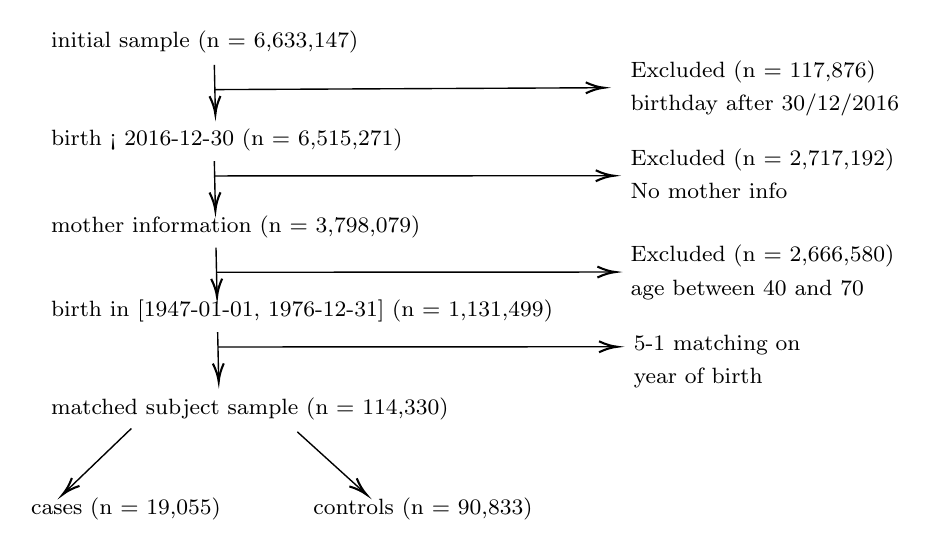
\begin{tikzpicture}[x=0.75pt,y=0.75pt,yscale=-0.8,xscale=0.8]
%uncomment if require: \path (0,327); %set diagram left start at 0, and has height of 327
%Straight Lines [id:da09755630118978076] 
\draw    (252,252) -- (292.15,288.41) ;
\draw [shift={(293.63,289.75)}, rotate = 222.2] [color={rgb, 255:red, 0; green, 0; blue, 0 }  ][line width=0.75]    (10.93,-3.29) .. controls (6.95,-1.4) and (3.31,-0.3) .. (0,0) .. controls (3.31,0.3) and (6.95,1.4) .. (10.93,3.29)   ;
%Straight Lines [id:da44638779412348717] 
\draw    (152,250) -- (112.08,288.36) ;
\draw [shift={(110.63,289.75)}, rotate = 316.14] [color={rgb, 255:red, 0; green, 0; blue, 0 }  ][line width=0.75]    (10.93,-3.29) .. controls (6.95,-1.4) and (3.31,-0.3) .. (0,0) .. controls (3.31,0.3) and (6.95,1.4) .. (10.93,3.29)   ;
%Straight Lines [id:da8871200673466652] 
\draw    (203,141) -- (203.59,168.75) ;
\draw [shift={(203.63,170.75)}, rotate = 268.78] [color={rgb, 255:red, 0; green, 0; blue, 0 }  ][line width=0.75]    (10.93,-3.29) .. controls (6.95,-1.4) and (3.31,-0.3) .. (0,0) .. controls (3.31,0.3) and (6.95,1.4) .. (10.93,3.29)   ;
%Straight Lines [id:da1648623506457928] 
\draw    (203.32,155.88) -- (441.63,155.75) ;
\draw [shift={(443.63,155.75)}, rotate = 179.97] [color={rgb, 255:red, 0; green, 0; blue, 0 }  ][line width=0.75]    (10.93,-3.29) .. controls (6.95,-1.4) and (3.31,-0.3) .. (0,0) .. controls (3.31,0.3) and (6.95,1.4) .. (10.93,3.29)   ;
%Straight Lines [id:da768775166366618] 
\draw    (204,192) -- (204.59,219.75) ;
\draw [shift={(204.63,221.75)}, rotate = 268.78] [color={rgb, 255:red, 0; green, 0; blue, 0 }  ][line width=0.75]    (10.93,-3.29) .. controls (6.95,-1.4) and (3.31,-0.3) .. (0,0) .. controls (3.31,0.3) and (6.95,1.4) .. (10.93,3.29)   ;
%Straight Lines [id:da9792209051883168] 
\draw    (204.32,200.88) -- (442.63,200.75) ;
\draw [shift={(444.63,200.75)}, rotate = 179.97] [color={rgb, 255:red, 0; green, 0; blue, 0 }  ][line width=0.75]    (10.93,-3.29) .. controls (6.95,-1.4) and (3.31,-0.3) .. (0,0) .. controls (3.31,0.3) and (6.95,1.4) .. (10.93,3.29)   ;
%Straight Lines [id:da7032136969785114] 
\draw    (202,89) -- (202.59,116.75) ;
\draw [shift={(202.63,118.75)}, rotate = 268.78] [color={rgb, 255:red, 0; green, 0; blue, 0 }  ][line width=0.75]    (10.93,-3.29) .. controls (6.95,-1.4) and (3.31,-0.3) .. (0,0) .. controls (3.31,0.3) and (6.95,1.4) .. (10.93,3.29)   ;
%Straight Lines [id:da2824593510407103] 
\draw    (202.32,45.88) -- (434.63,44.76) ;
\draw [shift={(436.63,44.75)}, rotate = 179.72] [color={rgb, 255:red, 0; green, 0; blue, 0 }  ][line width=0.75]    (10.93,-3.29) .. controls (6.95,-1.4) and (3.31,-0.3) .. (0,0) .. controls (3.31,0.3) and (6.95,1.4) .. (10.93,3.29)   ;
%Straight Lines [id:da6294357350000164] 
\draw    (202,31) -- (202.59,58.75) ;
\draw [shift={(202.63,60.75)}, rotate = 268.78] [color={rgb, 255:red, 0; green, 0; blue, 0 }  ][line width=0.75]    (10.93,-3.29) .. controls (6.95,-1.4) and (3.31,-0.3) .. (0,0) .. controls (3.31,0.3) and (6.95,1.4) .. (10.93,3.29)   ;
%Straight Lines [id:da5602976120653284] 
\draw    (202.32,97.88) -- (440.63,97.75) ;
\draw [shift={(442.63,97.75)}, rotate = 179.97] [color={rgb, 255:red, 0; green, 0; blue, 0 }  ][line width=0.75]    (10.93,-3.29) .. controls (6.95,-1.4) and (3.31,-0.3) .. (0,0) .. controls (3.31,0.3) and (6.95,1.4) .. (10.93,3.29)   ;

% Text Node
\draw (102,120) node [anchor=north west][inner sep=0.75pt]   [align=left] {\footnotesize mother information (n = 3,798,079)};
% Text Node
\draw (102,171) node [anchor=north west][inner sep=0.75pt]   [align=left] {\footnotesize birth in [1947-01-01, 1976-12-31] (n = 1,131,499)};
% Text Node
\draw (90,290) node [anchor=north west][inner sep=0.75pt]   [align=left] {\footnotesize cases (n = 19,055) };
% Text Node
\draw (260,290) node [anchor=north west][inner sep=0.75pt]   [align=left] {\footnotesize controls (n = 90,833)};
% Text Node
\draw (451,138) node [anchor=north west][inner sep=0.75pt]   [align=left] {\footnotesize Excluded (n = 2,666,580) \\\footnotesize age between 40 and 70};
% Text Node
\draw (102,230) node [anchor=north west][inner sep=0.75pt]   [align=left] {\footnotesize matched subject sample (n = 114,330)};
% Text Node
\draw (453,192) node [anchor=north west][inner sep=0.75pt]   [align=left] {\footnotesize 5-1 matching on \\\footnotesize year of birth};
% Text Node
\draw (102,9) node [anchor=north west][inner sep=0.75pt]   [align=left] {\footnotesize initial sample (n = 6,633,147)};
% Text Node
\draw (451,27) node [anchor=north west][inner sep=0.75pt]   [align=left] {\footnotesize Excluded (n = 117,876) \\\footnotesize birthday after 30/12/2016};
% Text Node
\draw (102,68) node [anchor=north west][inner sep=0.75pt]   [align=left] {\footnotesize birth < 2016-12-30 (n = 6,515,271)};
% Text Node
\draw (451,80) node [anchor=north west][inner sep=0.75pt]   [align=left] {\footnotesize Excluded (n = 2,717,192)\\\footnotesize No mother info};
\end{tikzpicture}
\caption{Consort flow chart for the construction of the Nested Case-Control dataset.}
\label{fig:nccd}
\end{figure}
\normalsize

We carry out a survival Cox model with the time-varying family history covariate $FH(t)$ on the NCCD \cite{zhang2018time}. The estimated relative risk results $RR = 1.8017$, which is aligned with the value from the literature equal to 1.8 \cite{collaborative2001familial, pharoah1997family}. This result validates the quality of our data. 

\subsection{Descriptive statistics}
Table \ref{tab:covsummaries} reports some descriptive statistics of the clean dataset composed by $4,267,803$ women, and only $n = 1,603,920$ when the term ``Red.'' accompanies the description. 

\begin{center}
\begin{table*}[!h]%
\begin{tabular*}{\textwidth}{@{\extracolsep\fill}lllll@{}}
    \toprule
    &Min. &Median &Mean &Max. \\ \cmidrule{2-5} 
    Birthday &1853-11-15 &1955-03-15 &1954-01-15 
    &2018-12-15 \\
    Diagnosis &1958-01-15 &1994-02-25 &1992-03-07 
    &2016-12-30  \\
    Death &1947-05-08 &1991-08-21 &1991-01-18 
    &2018-12-31  \\ 
    Emigration &1948-01-01 &1999-09-30 &1996-09-12 
    &2018-12-31 \\
    Age at diagnosis Red. &11.00 &50.00 &50.2 
    &69.00 \\
    Diagnosis Red. &1961-09-15 &2008-08-13 &2006-12-27 
    &2016-12-30 \\
    Death Red. &1948-10-25 &2006-12-26 &2000-08-10 
    &2018-12-31 \\
    Emigration Red. &1951-05-01 &1992-08-24 &1991-02-02 
    &2018-12-31 \\ \hline
    Follow-up (years) &0 &53.2922 &52.8118 
    &69.9576 \\ \midrule
    Breast cancer onset &Yes &No \\
    &47,914 (2.99\%) &1,556,006 (97.01\%) \\ \midrule
    EFS &Alive &Dead/emigrated &Diagnosed \\ 
    &1,408,072 (87.79\%) &147,914 (9.22\%) &47,934 (2.99\%) \\ \midrule
    & Yes & No \\
    FH at end of FU &105,432 (6.57\%) &1,498,488 (93.43\%) \\ 
    Parity &989,422 (38.31\%) &614,498 (61.69\%)    \\ \midrule
    &Min. &Median &Mean &Max. \\ 
    Number of children &1 &1 &1.5 &10 \\
    Age at first child &13.08 &27.25 &27.67 &60.33 \\ \bottomrule
    \end{tabular*}
    \caption{Summaries of the main variables obtained from the Multi-Generational Swedish dataset, where ``Red.'' refers to only the main subject (whose birthday ranges in [1947-01-01, 1976-12-31]); ``EFS'' means status at the end of the follow-up, ``FH'' means family history, and ``FU'' means follow-up.}
    \label{tab:covsummaries}
\end{table*}
\end{center}
% code in descriptiveStatistics.R from SWEDISH COMPUTER 

It is worth noting that the first recorded breast cancer diagnosis occurred in January 1958, with no specific day (we assume the onset date to be the 15th of that month). The final recorded case occurred on December 30th, 2016, providing a 58-year follow-up for analysis. We also consider this date as the end of the follow-up period. The median age at diagnosis is 50 years old, proving that the risk group that we select with ages in-between 40 and 70 is appropriate. This is reflected also in the median follow-up of around 53 years. Around the 3\% (47,934 subjects) have been diagnosed with invasive breast cancer, the 9.22\% are censored due to death, emigration or DCIS before the end of the follow-up, and the 87.79\% are alive at the end of the follow-up without experiencing neither breast cancer onset nor any other censoring events, so that we can consider this percentage as our cured fractions. Less than the 7\% has a positive family history at the end of the follow-up. For what concerns additional covariates that can be included into the models, the majority of women (61.69\%) is nulliparous, while, among those who have given birth, the average number of children is 1.5. The mean age at first child (27 years old) is appropriate for Sweden. Notice that all of these variables refer to the most recent follow-up time of the subject. Genetic factors and other details related to breast cancer are not available in the data, limiting the scope of our analysis to familial survival data provided by the women themselves during their visits. No medical tests or blood samples are available.

A majority of families (45.06\%) consist of two members, followed by three members (33.7\%) and four members (11.37\%). To provide complete information on family structure, we also report in Table \ref{tab:freqsis} the frequencies of sisters, as they play a critical role in our analysis. The first row of Table \ref{tab:freqsis} shows the percentage of families having a specific number of sisters for the ``main subjects'', where it can be observed that no main subject has precisely eleven sisters. The second row presents the cumulative percentage of sisters for the main subjects, which is equivalent to the non-missing information on the sister columns. For instance, the first row shows that 36$\%$ of main subjects have precisely one sister (``Freq.'' in the first column), while the 52\% have at least one sister (``Cum. Freq.'' in the second column).
\begin{center}
\begin{table*}[!h]%
\begin{tabular*}{\textwidth}{@{\extracolsep\fill}llllllllll@{}}
\toprule
    &\multicolumn{9}{c}{Number of sisters} \\\cmidrule{2-10} 
    % &(1, 0.8) 
    &0 &1 &2 &3 &4 &5 &6 &7 &$\ge$8  \\ \midrule % &(50, 10)
    Freq. &0.48 &0.36 &0.12 &0.03 &0.01 &3.1$\cdot10^{-3}$ &9$\cdot10^{-3}$ &0.0005 \\
    Cum. Freq.  &1 &0.52 &0.16 &0.04 &0.01 &0.005 &0.001 &0.0008 &0.0002 \\ 
    % Number of sisters & &9 &10 &11 &12 \\ 
    % Freq. &1$\cdot10^{-3}$ &3.8$\cdot10^{-4}$ &2.4$\cdot10^{-4}$ &- &0.06$\cdot10^{-4}$ \\
    % Cum. freq. &6.72$\cdot10^{-5}$ &2.92$\cdot10^{-5}$ &5.60$\cdot10^{-6}$ &5.60$\cdot10^{-6}$ \\ 
    \bottomrule
    \end{tabular*}
    \caption{Number of sisters of the main subjects.}
    \label{tab:freqsis}
% \end{sidewaystable}
\end{table*}
\end{center}
% Code from covariates.R in SWEDISH COMPUTER
% code in descriptiveStatistics.R from SWEDISH COMPUTER 

Once the dataset has been cleaned and merged across families and all necessary subject-specific information is collected, the observed time is determined based on whether the subject has experienced breast cancer onset, death, or emigration out of Sweden before in time. If the individual has not experienced any of these events, her observed time is the last day of the follow-up. The indicator of having observed the event follows immediately. In Figure \ref{fig:kmall}, we present the Kaplan-Meier estimator of the survival function for all subjects in the dataset, whose family size ranges from a minimum of one to a maximum of fourteen subjects. 
\begin{figure}[h]
    \centering
    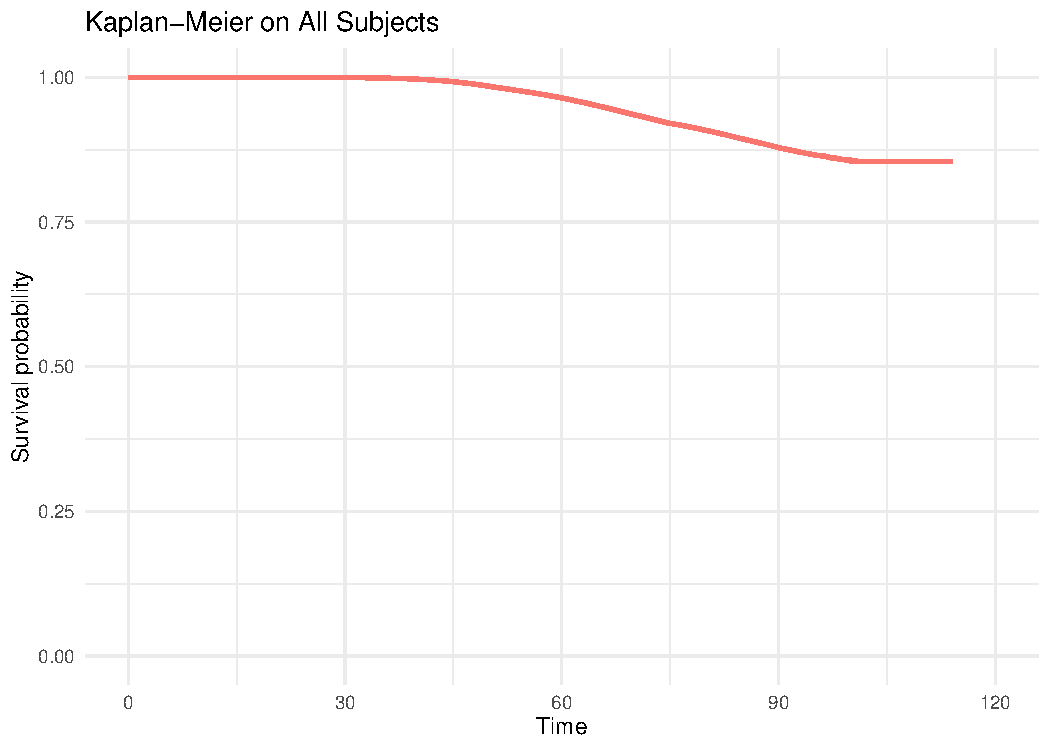
\includegraphics[width=\linewidth]{plots/Rplot100.pdf}
    \caption{Kaplan-Meier survival estimate of age at onset (all subjects).}
    \label{fig:kmall}
\end{figure}
% code in sisters.R SWEDEN COMPUTER  

Parameter estimation must be distinguished between the semiparametric and the parametric scenario. Notice that the analysis is conducted both on those main subjects that has a recorded mother in the Multi-Generational dataset and on all main subjects (with or without recorded mother in the dataset). A preliminary analysis on the covariate extension to parity indicator, number of children, and age at first child from Table \ref{tab:14}, is also conducted into the semiparametric setting. We plan to extend this preliminary analysis to a proper study of the inclusion of covariates into all models (both from semiparametric and parametric scenario), with a proper simulation study before the real case analysis.

\subsection{Semiparametric scenario}
In Section \ref{sec5} the Multivariate frailty Cox, the Univariate $FH$ Cox, and the Univariate $FH(t)$ Cox model have been analysed in simulation studies. Not surprisingly, based on the simulation results, the Multivariate frailty Cox model outperforms the others in terms of predictive accuracy. Similarly to simulation studies, also with the real case data the Multivariate frailty Cox model has a Concordance index of 0.965, which is significantly higher than the Univariate $FH$ Cox model (0.5150) and the Univariate $FH(t)$ Cox model with 0.5036 of concordance. All the results are reported in Table \ref{tab:13}. By selecting only the main subjects with a recorded mother into the dataset, the Concordance index almost reaches the maximum value, up to the 99\% of concordant pairs. This result is outstanding, and the advantage of using the Multivariate model instead of only the easier Univariate $FH$ model is immediately observed. Indeed, the Univariate $FH$ Cox and Univariate $FH(t)$ Cox models perform poorly, as their prediction concordance is comparable to that of a random flipping of a coin.
\begin{center}
\begin{table*}[!h]%
\begin{tabular*}{\textwidth}{@{\extracolsep\fill}lllll@{}}
\toprule
    &Survival information mother &$\widehat\theta$ &$\widehat\beta_{FH}$ &C \\ \cmidrule{2-5}
    Multivariate frailty Cox &yes &1.3624 &- &0.9968 \\
    Univariate $FH$ Cox &&- &1.5372 &0.5021 \\
    Univariate $FH(t)$ Cox &&- &1.8017 &0.5042 \\ \midrule
    Multivariate frailty Cox &no &1.327 &- &0.9650 \\
    Univariate $FH$ Cox &&- &1.449 &0.5150 \\ 
    Univariate $FH(t)$ Cox &&- &1.8405 &0.5036 \\ \bottomrule
    \end{tabular*}
    \caption{Estimated parameters and Harrell's concordance index (C).}
    \label{tab:13}
\end{table*}
\end{center}
% Code \texttt{finalEstimation-cox-swemultireg-MVV} in the Swedish VDI.

In Table \ref{tab:14} we report results from including the available reproductive covariates as parity, number of children, and age at first child. No significant differences in terms of Concordance index is noticed in comparison to the scenario without covariates.
\begin{center}
\begin{table*}[!h]%
\begin{tabular*}{\textwidth}{@{\extracolsep\fill}lllll@{}}
\toprule
    &Survival information mother &$\widehat\theta$ &$\widehat{\beta}_{FH}$ &C \\ \cmidrule{2-5}
    Multivariate &yes &2 &- &0.9335 \\
    Univariate FH &&- &1.3922 &0.6209 \\
    Univariate FH(t) &&- &2.2254 &0.5350 \\ \midrule
    Multivariate &no &2 &- &0.9436 \\
    Univariate FH &&- &1.3922 &0.5965 \\ 
    Univariate FH(t) &&- &1.8049 &0.5184 \\ \bottomrule
    \end{tabular*}
    \caption{Estimated parameters and Harrell's concordance index (C) for the models with parity, number of children, and age at first child.}
    \label{tab:14}
\end{table*}
\end{center}
% Code \texttt{finalEstimationCovariates-cox-swemultireg-MVV} in the SWEDISH COMPUTER.
% Code in ParContinuousFrailty-multivariate-swemultireg-MVV.R in the SWEDISH COMPUTER for the estimation of parameters and ParContinuousFrailty-multiunifh-postprediction-swemultireg-MVV.R for concordance with adjustement on the parameter values. 

Notice that the estimated family history coefficient $\widehat{\beta}_{FH}$ has a positive value (around 1.8) meaning that the family history has a positive effect on the breast cancer development, that is indeed coherent with the literature.  

We then use the estimated parameters to perform posterior prediction of family-specific frailty risk. 
%Firstly, we apply the posterior prediction to the subjects in the initial dataset. Secondly, we perform an in-sample validation to assess the accuracy of the prediction. This involves defining a training and a validation set by conducting a in-sample validation. 
% Specifically, we remove one family at a time, fit the model on the remaining (n - 1) families, and predict only on the excluded family using the previously estimated parameters.

We compute an algorithm which takes as input the familial survival data of the female family members of a new woman. By providing information on her mother and sisters, the algorithm produces three quantities: the posterior mean frailty risk, the probability of belonging to the highest-risk families (top 5\%), and an indicator of whether the woman belongs to the highest-risk families compared to the population (prior) distribution of the probability of belonging to the highest-risk families, based on a fixed threshold. For example, from the Multivariate frailty Cox model we obtain that $\widehat{\theta} = 1.327$, and $\widehat{r}_{(1-\alpha)}$ is $0.1512$ for $\alpha = 0.05$. This means that if a woman has a probability of belonging to the highest-risk families over 15.12\%, then her indicator will take value one. Risk prediction can be easily done by using the estimated frailty parameter, the (1-$\alpha$) percentile value, and also the Breslow estimates of the cumulative hazard function obtained by fitting the Multivariate frailty Cox model. These values can be stored for later use, enabling fast prediction without having to recompute the entire process for new women. This algorithm has been developed based on the model chosen in Section \ref{sec5}.

In Table \ref{tab:17} a summary of the distribution of the cumulative hazard function is provided. The plot of the  cumulative hazard function and its density function on the complete population are respectively in Figure \ref{fig:8} and \ref{fig:9}. Interestingly, we can notice how the density function can be split into two regions. It is straightforward to extend this procedure to other percentile levels, although this necessitates refitting the model from the beginning, which can be time-consuming. On the other hand, every computation can be done for once and store it for a later use.
\begin{center}
\begin{table*}[!h]%
\begin{tabular*}{\textwidth}{@{\extracolsep\fill}lllllll@{}}
\toprule
    Min. &1st Qu. &Median &Mean &3rd Qu. &Max. &NA's \\ \midrule
    0.0000  &0.0000 &0.0324 &0.0752 &0.1389 &0.2583 &360 \\ \bottomrule
    \end{tabular*}
    \caption{Summary of the estimated Breslow cumulative hazard function on a grid of (time) values.}
    \label{tab:17}
\end{table*}
\end{center}
\begin{figure}
    \centering
    \includegraphics[width=\linewidth]{PhD_thesis_template/plots/Rplot107.pdf}
    \caption{Estimated Breslow cumulative hazard function.}
    \label{fig:8}
\end{figure}
\begin{figure}
    \centering\includegraphics[width=\linewidth]{PhD_thesis_template/plots/Rplot102.pdf}
    \caption{Density plot of the Breslow cumulative hazard function estimated on the entire population in object.}
    \label{fig:9}
\end{figure}
An example of risk prediction into the semiparametric scenario is reported below for a woman with complete family survival information. Observed ages = (45, 90, 60) in years, and indicators of having observed the onset event = (0, 1, 0). Consider the first subject to be the woman who shows up at the hospital at 45 years of age, with the mother who had breast cancer onset at 90, and a sister who has not experienced the onset yet at age 60. The output from the algorithm below means that the woman has a frailty risk with value 1.57 if estimated through the posterior mean; with value 2.78 if estimated through the posterior median. She also has a probability of belonging to the highest-risk families of 12.64\% that is slower than the top 5\% threshold of 15.12\% and thus she does not belong to the highest-risk families. All the quantities can be found in the following output: \\
\begin{verbatim}
    Posterior mean frailty = 1.5762
    Posterior median frailty = 2.7801
    Posterior high-risk probability = 0.1264
    Posterior high-risk membership = 0
\end{verbatim}
% Code with name \texttt{postPredictionReal1Family} and in Appendix \ref{appendix:b}. 

It is worth noting that in the parametric scenario, the population parametric distribution provides more information and therefore there is no requirement for computing the nonparametric estimates of the cumulative hazard function and the quantile threshold. 
 
\subsection{Parametric scenario}
The Swedish real case dataset also provides us with a precious opportunity to explore the debated issue of whether a cure-rate structure is reasonable in models for breast cancer onset or not. 

We first focus on the goodness of fit of Cure-Rate models versus traditional models to the available dataset, to give a qualitative support to the hypothesis that a cured fraction exists and the Cure-Rate models are able to capture it. Notice that, in this preliminary analysis, the frailty quantity has not been involved yet. We employee five parametric distributions: Weibull, Gamma, Lognormal, three-parameter Gamma, and three-parameter Lognormal for the baseline survival function of cases. 

Results from the analysis are presented in Table \ref{tab:10}, where the models are compared using the Akaike Information Criterion (AIC) that is exactly \[
AIC = -2 n_{\pi} - \ln L(\pi),
\] where $n_\pi$ is the dimension of the parameter collection, and $L(\pi)$ is the likelihood on the parameter collection. It should be noted that the models are not nested. We compare the fit across the several survival function distributions, and also between the cure-rate and non-cure-rate survival structure but always within the multivariate and the univariate cases (which also have very different sample sizes). The Multivariate Cure-Rate three-parameter Lognormal model yields the best result, with an AIC value of 1687555, while the regular Lognormal distribution provides the best performance for the Univariate Cure-Rate model with an AIC of 438368.4. From results, the cure-rate models are always preferred to the non-cure-rate models (except for the case of the Multivariate Lognormal model).

All the curves shown in Figures \ref{fig:1.13}, \ref{fig:1.14}, and \ref{fig:1.15} support the hypothesis of involving a cure-rate model rather than a (traditional) non-cure model. Indeed, the cure-rate model seems to fit the data (until the end of the follow-up) better than the non-cure models. 

It is interesting to notice that support to the cure-rate structure is mainly given by the graphical analysis of the survival function of the mothers, due to their older ages: in Figure \ref{kmsisters}, the Kaplan-Meier curves by subjects (the main subject, the mother, and from the first sister to the last one) show that the tail of the Kaplan-Meier estimator and of the fitted cure-rate models (Figure \ref{fig:1.13}, \ref{fig:1.14}, \ref{fig:1.15}) is mostly attributable by the mothers (in black). A deepening about the reliability of the cure-rate structure and the heavy tail due to the presence of the oldest mothers is in Appendix \ref{appendix:1.e}. We do not find particular graphical differences in curves among the daughters, as it should be expected since the main subject is randomly sampled among all the sisters. One might extend the models to allow for a (say, polynomial) effect of birth cohort on the survival distribution and make distinction between the mother and the sisters.
\begin{center}
\begin{table*}
\begin{tabular*}{\textwidth}{@{\extracolsep\fill}lll@{}}
\toprule 
    &\multicolumn{2}{c}{Survival function} \\ \cmidrule{2-3}
    &non-cure &cure-rate \\ \midrule
    Multivariate model \\
    Weibull &1705353 &1692822 \\ 
    Gamma &1698245 &1688066 \\ 
    Lognormal &1693854 &2334626 \\ 
    three-parameter Gamma &1707589 &1687749 \\
    three-parameter Lognormal &1698257 &1687555 \\ \midrule
    Univariate model \\ 
    Weibull &440685.6 &439053.4 \\ 
    Gamma &439516 &438391.8 \\
    Lognormal &438958.8 &438368.4 \\ 
    Gamma 3-parameters &444890.7 &438386.2 \\
    Lognormal 3-parameters &439460.9 &438369 \\ \bottomrule
\end{tabular*}
\caption{AIC comparison among different survival distributions.}
\label{tab:10}
\end{table*}
\end{center}
% Code in oneGroupGamma.R, oneGroupLogNormal.R, oneGroupWeibullNecessary.R in SWEDISH COMPUTER

\begin{figure}
    \centering
    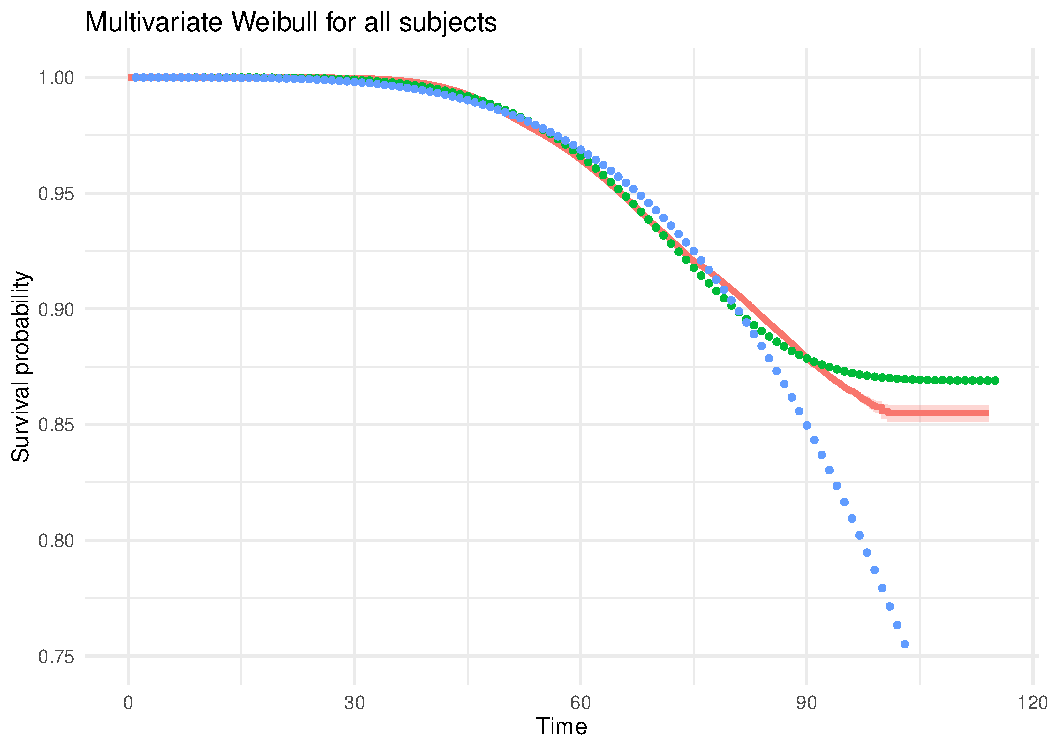
\includegraphics[width=\linewidth]{PhD_thesis_template/plots/Rplot108.pdf}
    \includegraphics[width=\linewidth]{PhD_thesis_template/plots/Rplot109.pdf}
   \caption{Kaplan-Meier for all subjects, in comparison to the estimated survival curves following the cure-rate (green) and the non-cure (blue) survival structure with Weibull and Gamma baseline survival function, on top and below, respectively.}
    \label{fig:1.13}
\end{figure}
\begin{figure}
    \centering
    \includegraphics[width=\linewidth]{plots/Rplot111.pdf}
        \includegraphics[width=\linewidth]{plots/Rplot112.pdf}
    \caption{Kaplan-Meier for all subjects, in comparison to the estimated survival curves following the cure-rate (green) and the non-cure (blue) survival structure, with Lognormal and three-parameter Lognormal survival function, on top and below, respectively.}
    \label{fig:1.14}
\end{figure}
\begin{figure}
    \centering
    \includegraphics[width=\linewidth]{plots/Rplot110.pdf}
    \caption{Kaplan-Meier for all subjects, in comparison to the estimated survival curves following the cure-rate (green) and the non-cure (blue) survival structure, with a three-parameter Gamma baseline survival function.}
    \label{fig:1.15}
\end{figure}
% Code for these plots is in: KMSubjectsMothers_Ultracentenary.R in the Swedish computer. 
\begin{figure}[ht]
    \centering
    \includegraphics[width=\linewidth]{plots/Rplot106.pdf}
    \caption{Kaplan-Meier of daughters and mother (in black).}
    \label{kmsisters}
\end{figure}
% code in sisters.R SWEDEN COMPUTER 

Once proved that the cure-rate model is the most appropriate for describing this real case dataset, we proceed to parameter estimation. We report the values of the estimated parameters in Table \ref{tab:1.17} and \ref{tab:1.18}. We run the analysis both on main subjects with a recorded mother in the registry or on main subjects without restrictions. In Table \ref{tab:1.17} the survival function has a Weibull distribution. On the contrary, in Table \ref{tab:1.18} we extend to different baseline survival distributions on all the main subjects. The estimated cured fraction value has a reasonable value for this specific application in the range around 87\%-96\% for $\widehat p$ in the first column of Table \ref{tab:1.17}. The tables also report the estimates of the baseline survival distribution parameters, that are $\widehat shape_0$, and $\widehat scale_0$ for the Weibull and Gamma, with the addition of $\widehat\gamma_0$ for the threshold parameter in the three-parameter Gamma; $\widehat\mu_0$, and $\widehat\sigma^2_0$ for the Lognormal, with the addition of $\widehat\gamma_0$ for the threshold parameter in the three-parameters Lognormal. The frailty parameter $\widehat\theta$ and the $FH$ coefficient $\widehat{\beta}_{FH}$ are reported in the same column because estimating one of the two exclude the estimation of the other. Notice that only the models with ``FH'' in the name estimate the family history coefficient $\beta_{FH}$.
\begin{center}
\begin{table*}[!h]%
\begin{tabular*}{\textwidth}{@{\extracolsep\fill}lllllll@{}}
    \toprule
    &Survival info mother &$\widehat p$ &$\widehat{shape}_0$ &$\widehat{scale}_0$ &$\widehat\theta$/$\widehat{\beta}_{FH}$ &C \\ \cmidrule{2-7}
    MFCR &yes &0.8710  &6.2645 &73.2018  &4.9053 &0.9592 \\
    UFCR &&0.9594 &0.1246 &0.1900 &1.2150 &0.3952 \\
    U$FH$CR &&0.9635 &0.0926 &0.0394 &1.2174 &- \\ \midrule
    MFCR &no &0.8703  &6.1822 &72.9776  &4.3569 &0.9663 \\
    UFCR &&0.9750 &0.1176 &0.1193 &1.2614 &0.3963 \\  
    U$FH$CR &&0.9658 &0.0965 &0.0362 &1.1982 &- \\ \midrule
    \end{tabular*}
    \caption{Estimated parameters and Concordance index for the Multivariate frailty Cure-Rate (MFCR), the Univariate frailty Cure-Rate (UFCR), and the Univariate $FH$ Cure-Rate (U$FH$CR) models.}
    \label{tab:1.17}
\end{table*}
\end{center}
% Code in ParContinuousFrailty-multidistribution-multivariate-swemultireg-MVV.R, ParContinuousFrailty-multidistribution-univariate-swemultireg-MVV.R, ParContinuousFrailty-multidistribution-univariate-fh-swemultireg-MVV.R in the SWEDISH COMPUTER for the estimation of parameters and ParContinuousFrailty-multiunifh-postprediction-swemultireg-MVV.R for concordance with adjustement on the parameter values.  
\begin{center}
\begin{table*}[!h]%
\begin{tabular*}{\textwidth}{@{\extracolsep\fill}lllllll@{}}
    \toprule
    &$\widehat p_0$ &$\widehat\mu_0 / \widehat{shape}_0$ &$\widehat\sigma^2_0 / \widehat{scale}_0$ &$\widehat\gamma_0$ &$\widehat\theta$/$\widehat{\beta}_{FH}$ &C \\ \cmidrule{2-7}
    Multivariate frailty Cure-Rate \\
    Weibull &0.8703  &6.1822 &72.9776 &- &4.3569 &0.9663 \\ 
    Gamma &0.8552 &18.6981  &3.8617 &- &5.4790 &0.9663 \\ 
    Lognormal &0.8419 &4.2911 &0.2604 &- &5.5265 &0.9392 \\ 
    Gamma 3-pars &0.8529 &18.6685 &3.8172 &0.1546 &5.8116 &0.9679 \\
    Lognormal 3-pars &0.8408 &4.2746 &0.2590 &2.7922 &5.9126 &0.9663 \\ \hline
    Univariate frailty Cure-Rate \\
    Weibull &0.9750 &0.1176 &0.1193 &- &1.2614 &0.3963 \\ 
    Gamma &0.8626 &5.9127 &11.5267 &- &-5.8713 &0.3963 \\ 
    Lognormal &0.6607 &4.5317 &0.3784 &- &1.4119 &0.5105 \\ 
    Gamma 3-pars &0.3250 &9.5974 &11.0534 &3.1358 &-1.4014 &0.4461 \\
    Lognormal 3-pars &0.2527 &4.8125 &0.4431 &11.5269 &2.0759 &0.4900 \\ \hline
    Univariate FH \\
    Weibull &0.9635 &0.0926 &0.0394 &- &1.2174 &- \\ 
    Gamma &0.9590 &22.0724  &2.5169 &- &-1.1910 &- \\ 
    Lognormal &0.9774 &2.6356 &0.9717 &- &-3.0954 &- \\ 
    Gamma 3-pars &0.7076 &11.8656 &6.9557 &0.5153 &0.7802 &- \\
    Lognormal 3-pars &0.5237 &4.6639 &0.4117 &7.9716 &2.0892 &- \\ \hline
    \end{tabular*}
    \caption{Estimated parameters for several baseline survival distribution for cases.}
    \label{tab:1.18}
\end{table*}
\end{center}
% codice su server meb: ParContinuousFrailty-multidistribution-multivariate-swemultireg-MVV.R, ParContinuousFrailty-multidistribution-univariate-swemultireg-MVV.R, ParContinuousFrailty-multidistribution-univariate-fh-swemultireg-MVV.R and ParContinuousFrailty-multiunifh-postprediction-swemultireg-MVV.R for concordance with adjustement on the parameter values. 
%  code for concordance multi-uni-unifh is in prova-concordance-2.R SWEDEN 

Similarly to the semiparametric scenario, the multivariate model outperforms the other two univariate models compared in terms of prediction accuracy through the Harrell's concordance index C, reported in the last column of Tables \ref{tab:1.17}, and \ref{tab:1.18}. It has indeed around the 96\% of concordant pairs. Also, in comparison to the semiparametric scenario we can say that the estimated frailty parameter has a higher value in the multivariate parametric scenario bringing to assess that the frailty distribution here has a higher variance and thus this brings to an easier distinction among low-risk and higher-risk families, than the semiparametric scenario. 

Now we can predict the posterior family-specific frailty as shown in Section \ref{sec:1.6}. We compute the mean, median and mode of the posterior frailty distribution for each family. Later, we compute the posterior high-risk probability and the posterior high-risk membership indicator, fixed a frailty mean threshold. Here, too, we can also compute the whole estimated family-specific survival distribution, conditionally on the family survival information. For each woman we can compute thus, as in the semiparametric scenario, all the interesting quantities to assess whether to address her to prevention strategies targeted for highest-risk families. 
\clearpage

\section{Discussion}\label{sec:1.7}
This study aims to contribute to the study of risk prediction models for breast cancer to better understand the nature and modeling of family-specific risk of onset. We consider the cure-rate structure as a realistic approach for the Swedish Multi-Generational Breast Cancer registry, where around the 85$\%$ of subjects have not experienced yet breast cancer onset within the observed follow-up. We thus extend the traditional proportional hazards assumption in this Lehmann family formulation to cure-rate models. We explore parametric (Gamma shared frailty) models in this cure-rate setting, as well as semiparametric models that do not assume the cure-rate structure. 

Although family information is crucial for risk prediction models for breast cancer, using only a summary of this information may not have enough predictive power, as it proved with the often used family history indicator (baseline covariate, or time-varying covariate). Our simulation-based comparison shows that a full multivariate framework induces much better performance in terms of accuracy in risk prediction, when only involving family membership without additional subject-specific covariates. A full assessment of the added value of the full multivariate model will clearly emerge when additional analyses can be conducted on other dataset. Including family-specific covariates can enhance precision in targeting and improve accuracy in identifying the frailty parameter, as well as classifying families into risk groups. Therefore, incorporating family-specific covariates is an intriguing extension worth exploring.

We believe that this work stands out among the others known in the literature as it improves several aspects of breast cancer risk prediction models. We report a deep comparison between our model and the BOADICEA model, that is one of the most powerful in this context. 

The BOADICEA model is based on a multiplicative hazard function that depends on a genetic frailty component. This approach consists of inferring a genetic latent quantity, the polygenic risk score (PRS), for predicting cancer risk based on the family history of the disease and other risk factors. The PRS is a weighted combination of single nucleotide polymorphisms (SNPs), which are genetic mutations, commonly spread into the population, that singularly give a small contribution to increase the risk of breast cancer, but that can be dangerous when combined all together.

The BOADICEA model is then univariate and based on the subject-specific hazard function \[ \lambda(t\mid r) = \lambda_0(t)exp(\beta(r)), \] as described in detail in several publications (\cite{antoniou2002comprehensive}, \cite{antoniou2004boadicea}, \cite{antoniou2008boadicea}, and \cite{thomas2004statistical}). It evaluates the likelihood function through a complex segregation analysis provided by the Mendel software \cite{lee2019boadicea}. 

In contrast, our proposed frailty model differs from the BOADICEA model (or other possible similar models) in several ways. While BOADICEA uses a subject-specific hazard within a univariate framework and infers a genetic latent quantity, our model works in a fully multivariate framework and we infer a generic risk latent quantity, i.e. the subject-specific polygenic score. We incorporate survival information in a family-specific hazard, while the BOADICEA hazard function is subject-specific and does not account explicitly for the family structure through the estimated genetic frailty component. Our model wins in the simplicity that it has involving only familial breast cancer information and no other factors such as genetic, as BOADICEA does. Nevertheless, it is not difficult to extend our work to the use of additional  covariates. The simplicity is also extended to the use of a full likelihood or partial likelihood maximization algorithm for parameter estimation, while BOADICEA relies on a complex segregation analysis to predict the PRS (specifically its variance).

Last but not least, at contrary to the BOADICEA model, we introduce the explicit cure-rate structure on the survival function, that is crucial when especially dealing with breast cancer risk prediction models.

Talking about possible extensions of our work, one could be the use of alternative frailty distributions, such as the Lognormal \cite{duchateau2008frailty}. Or, one could address the problem within the Bayesian framework \cite{karamoozian2021bayesian}. One could also compare the prediction accuracy between our multivariate -- semiparametric and parametric -- model and the BOADICEA model, but it would be necessary the access to the same complete dataset \cite{lee2017differences}.

% The method with the multivariate model is able to identify higher-risk families to address them to targeted screening surveillance and prevention paths.

% The family information has been proved to be crucial to gain more information on the risk of having breast cancer. The Univariate model has been proved to be not useful for this topic. The model is not identifiable so far, without the inclusion of valid familiar covariates. Of course this work can be readily extended to the use of covariates and compare again the multivariate model with the univariate to assess whether the available covariates could be useful for knowing the familiar risk to breast caner. The issue with this dataset is that we have not precise familiar information, but we can build some as the number of people in the family or the number of sons. 

% Unfortunately all the families are from Sweden and they are registered as Swedish citizen so we can not distinguish among countries. Also other information are equivalent over all the families and indeed not useful. Without covariates, the multivariate model not only performs better than the univariate model because it uses the survival family information but also it is more powerful than the family history indicator in terms of prediction accuracy. The family history indicator uses as well the family information but in a simplistic way, indeed we can appreciate, through this study, the huge advantage in using the extended family information instead of just a summary. 

% The adjusted mean results to be correlated to the real frailty in the simulation studies, but the summary error index related to the regular mean is always lower according the every family size maximum/minimum. This means that we prefer to use an index that is closer to the real frailty, and indeed the mean is used in the application. 

% There is shrinkage towards one when the expected number of events is very low. There a large amount of shrinkage in the cure-rate model when the families have few members within. It is interesting to study the behaviour of the posterior estimator of the frailty close to zero because the shrinkage is heavily towards the mean in our case. 

% compile first the main.tex, then run Bibtex on Chapter1.bib, Chapter2.bib and Chapter3.bib, finally compile main.tex again twice
\clearpage
\renewcommand{\bibname}{References}
\bibliographystyle{apalike}
\bibliography{biblio}
